%  LaTeX support: latex@mdpi.com 
%  In case you need support, please attach all files that are necessary for compiling as well as the log file, and specify the details of your LaTeX setup (which operating system and LaTeX version / tools you are using).

%=================================================================
\documentclass[data,datadescriptor,accept,moreauthors,pdftex]{Definitions/mdpi} 

% If you would like to post an early version of this manuscript as a preprint, you may use preprint as the journal and change 'submit' to 'accept'. The document class line would be, e.g., \documentclass[preprints,article,accept,moreauthors,pdftex]{mdpi}. This is especially recommended for submission to arXiv, where line numbers should be removed before posting. For preprints.org, the editorial staff will make this change immediately prior to posting.

%--------------------
% Class Options:
%--------------------
%----------
% journal
%----------
% Choose between the following MDPI journals:
% acoustics, actuators, addictions, admsci, aerospace, agriculture, agriengineering, agronomy, algorithms, animals, antibiotics, antibodies, antioxidants, applsci, arts, asc, asi, atmosphere, atoms, axioms, batteries, bdcc, behavsci , beverages, bioengineering, biology, biomedicines, biomimetics, biomolecules, biosensors, brainsci , buildings, cancers, carbon , catalysts, cells, ceramics, challenges, chemengineering, chemistry, chemosensors, children, cleantechnol, climate, clockssleep, cmd, coatings, colloids, computation, computers, condensedmatter, cosmetics, cryptography, crystals, dairy, data, dentistry, designs , diagnostics, diseases, diversity, drones, econometrics, economies, education, ejihpe, electrochem, electronics, energies, entropy, environments, epigenomes, est, fermentation, fibers, fire, fishes, fluids, foods, forecasting, forests, fractalfract, futureinternet, futurephys, galaxies, games, gastrointestdisord, gels, genealogy, genes, geohazards, geosciences, geriatrics, hazardousmatters, healthcare, heritage, highthroughput, horticulturae, humanities, hydrology, ijerph, ijfs, ijgi, ijms, ijns, ijtpp, informatics, information, infrastructures, inorganics, insects, instruments, inventions, iot, j, jcdd, jcm, jcp, jcs, jdb, jfb, jfmk, jimaging, jintelligence, jlpea, jmmp, jmse, jnt, jof, joitmc, jpm, jrfm, jsan, land, languages, laws, life, literature, logistics, lubricants, machines, magnetochemistry, make, marinedrugs, materials, mathematics, mca, medicina, medicines, medsci, membranes, metabolites, metals, microarrays, micromachines, microorganisms, minerals, modelling, molbank, molecules, mps, mti, nanomaterials, ncrna, neuroglia, nitrogen, notspecified, nutrients, ohbm, optics, particles, pathogens, pharmaceuticals, pharmaceutics, pharmacy, philosophies, photonics, physics, plants, plasma, polymers, polysaccharides, preprints , proceedings, processes, proteomes, psych, publications, quantumrep, quaternary, qubs, reactions, recycling, religions, remotesensing, reports, resources, risks, robotics, safety, sci, scipharm, sensors, separations, sexes, signals, sinusitis, smartcities, sna, societies, socsci, soilsystems, sports, standards, stats, surfaces, surgeries, sustainability, symmetry, systems, technologies, test, toxics, toxins, tropicalmed, universe, urbansci, vaccines, vehicles, vetsci, vibration, viruses, vision, water, wem, wevj

%---------
% article
%---------
% The default type of manuscript is "article", but can be replaced by: 
% abstract, addendum, article, benchmark, book, bookreview, briefreport, casereport, changes, comment, commentary, communication, conceptpaper, conferenceproceedings, correction, conferencereport, expressionofconcern, extendedabstract, meetingreport, creative, datadescriptor, discussion, editorial, essay, erratum, hypothesis, interestingimages, letter, meetingreport, newbookreceived, obituary, opinion, projectreport, reply, retraction, review, perspective, protocol, shortnote, supfile, technicalnote, viewpoint
% supfile = supplementary materials

%----------
% submit
%----------
% The class option "submit" will be changed to "accept" by the Editorial Office when the paper is accepted. This will only make changes to the frontpage (e.g., the logo of the journal will get visible), the headings, and the copyright information. Furthermore, line numbering will be removed. Journal info and pagination for accepted papers will also be assigned by the Editorial Office.

%------------------
% moreauthors
%------------------
% If there is only one author the class option oneauthor should be used. Otherwise use the class option moreauthors.

%---------
% pdftex
%---------
% The option pdftex is for use with pdfLaTeX. If eps figures are used, remove the option pdftex and use LaTeX and dvi2pdf.

%=================================================================
\firstpage{1} 
\makeatletter 
\setcounter{page}{\@firstpage} 
\makeatother
\pubvolume{xx}
\issuenum{1}
\articlenumber{5}
\pubyear{2020}
\copyrightyear{2020}
%\externaleditor{Academic Editor: name}
\history{Received: 10 April 2020; Accepted: 13 May 2020; Published: date}
\updates{yes} % If there is an update available, un-comment this line

%% MDPI internal command: uncomment if new journal that already uses continuous page numbers 
%\continuouspages{yes}

%------------------------------------------------------------------
% The following line should be uncommented if the LaTeX file is uploaded to arXiv.org
%\pdfoutput=1

%=================================================================
% Add packages and commands here. The following packages are loaded in our class file: fontenc, calc, indentfirst, fancyhdr, graphicx, lastpage, ifthen, lineno, float, amsmath, setspace, enumitem, mathpazo, booktabs, titlesec, etoolbox, amsthm, hyphenat, natbib, hyperref, footmisc, geometry, caption, url, mdframed, tabto, soul, multirow, microtype, tikz
%% Additional packages
\usepackage{standalone}
\usepackage{listings}
\usepackage{xcolor}
\usepackage{rotating}
\usepackage{tikzpeople}
\usepackage{makecell}
% \usepackage{refcheck} % debuging
% code
\lstset{
    language = R,
    basicstyle = \small\ttfamily,
    stringstyle = \color{orange},
    % key words
    otherkeywords = {0,1,2,3,4,5,6,7,8,9},
    morekeywords = {TRUE,FALSE},
    keywordstyle = \color{blue},
    % comments
    commentstyle = \color{darkgray},
    morecomment = [f][\color{red}][0]{\#},
    % frame
    frame = single,
    backgroundcolor = \color{white}
}
% tikz
\usetikzlibrary{trees,
                arrows,
                shapes.geometric,
                positioning,
                calc,
                backgrounds,
                fit}

%=================================================================
%% Please use the following mathematics environments: Theorem, Lemma, Corollary, Proposition, Characterization, Property, Problem, Example, ExamplesandDefinitions, Hypothesis, Remark, Definition, Notation, Assumption
%% For proofs, please use the proof environment (the amsthm package is loaded by the MDPI class).

%=================================================================
% Full title of the paper (Capitalized)
\Title{Standartox: Standardizing Toxicity Data}

% Author Orchid ID: enter ID or remove command
\newcommand{\orcidauthorA}{0000-0002-9290-3965} % Add \orcidA{} behind the author's name
\newcommand{\orcidauthorB}{0000-0001-8732-3766} % Add \orcidB{} behind the author's name
\newcommand{\orcidauthorC}{0000-0003-3510-1701} % Add \orcidB{} behind the author's name

% Authors, for the paper (add full first names)
\Author{\hl{Andreas} Scharmüller$^{1,2,}$*\orcidA{}, Verena C. Schreiner $^{1}$\orcidB and Ralf B. Schäfer $^{1}$\orcidC{}}%Please carefully check the accuracy of names and affiliations. Changes will not be possible after proofreading. 

% Authors, for metadata in PDF
\AuthorNames{Andreas Scharmüller, Verena C. Schreiner and Ralf B. Schäfer}

% Affiliations / Addresses (Add [1] after \address if there is only one affiliation.)
\address{%
$^{1}$ \quad iES Landau, Institute for Environmental Sciences, University of Koblenz-Landau,
D-76829 Landau, Germany; scharmueller@uni-landau.de (A.S.); schreiner-verena@uni-landau.de (V.C.S.); schaefer-ralf@uni-landau.de (R.B.S.)\\
$^{2}$ \quad Laboratoire d’Hydrologie et de Géochimie de Strasbourg, UMR 7517 CNRS-Université de Strasbourg, \mbox{1 rue Blessig,} 67084 Strasbourg CEDEX, France}

% Contact information of the corresponding author
\corres{Correspondence: andschar@protonmail.com}

% Current address and/or shared authorship
% \firstnote{Current address: Affiliation 3} 
% \secondnote{These authors contributed equally to this work.}
% The commands \thirdnote{} till \eighthnote{} are available for further notes

%\simplesumm{} % Simple summary

%\conference{} % An extended version of a conference paper

% Abstract (Do not insert blank lines, i.e., \\) 
\abstract{An increasing number of chemicals such as pharmaceuticals, pesticides and synthetic hormones are in daily use all over the world. In the environment, chemicals can adversely affect populations and communities and in turn related ecosystem functions. To evaluate the risks from chemicals for ecosystems, data on their toxicity, which are typically produced in standardized ecotoxicological laboratory tests, is required. The results from ecotoxicological tests are compiled in (meta-)databases such as the United States Environmental Protection Agency (EPA) ECOTOXicology Knowledgebase (ECOTOX). However, for many chemicals, multiple ecotoxicity data are available for the same test organism. These  can vary strongly, thereby causing uncertainty of related analyses. Given that most current databases lack aggregation steps or are confined to specific chemicals, we developed Standartox, a tool and database that continuously incorporates the ever-growing number of test results in an automated process workflow that ultimately leads to a single aggregated data point for a specific chemical-organism test combination, representing the toxicity of a chemical. Standartox can be accessed through a web application and an R~package.}%website is not allowed in abstract %AS done

% Keywords
\keyword{ecotoxicology; standardization; environmental risk assessment; effect database; database; software; R; API} % up to 10

% The fields PACS, MSC, and JEL may be left empty or commented out if not applicable
%\PACS{J0101}
%\MSC{}
%\JEL{}

%%%%%%%%%%%%%%%%%%%%%%%%%%%%%%%%%%%%%%%%%%
% Only for the journal Diversity
%\LSID{\url{http://}}

%%%%%%%%%%%%%%%%%%%%%%%%%%%%%%%%%%%%%%%%%%
% Only for the journal Applied Sciences:
%\featuredapplication{Authors are encouraged to provide a concise description of the specific application or a potential application of the work. This section is not mandatory.}
%%%%%%%%%%%%%%%%%%%%%%%%%%%%%%%%%%%%%%%%%%

%%%%%%%%%%%%%%%%%%%%%%%%%%%%%%%%%%%%%%%%%%
% Only for the journal Data:
%\dataset{DOI number or link to the deposited data set in cases where the data set is published or set to be published separately. If the data set is submitted and will be published as a supplement to this paper in the journal Data, this field will be filled by the editors of the journal. In this case, please make sure to submit the data set as a supplement when entering your manuscript into our manuscript editorial system.}
\dataset{\url{https://doi.org/10.5281/zenodo.3785031}}


%\datasetlicense{license under which the data set is made available (CC0, CC-BY, CC-BY-SA, CC-BY-NC, etc.)}
\datasetlicense{MIT}

%%%%%%%%%%%%%%%%%%%%%%%%%%%%%%%%%%%%%%%%%%
% Only for the journal Toxins
%\keycontribution{The breakthroughs or highlights of the manuscript. Authors can write one or two sentences to describe the most important part of the paper.}

%\setcounter{secnumdepth}{4}
%%%%%%%%%%%%%%%%%%%%%%%%%%%%%%%%%%%%%%%%%%
\begin{document}
%%%%%%%%%%%%%%%%%%%%%%%%%%%%%%%%%%%%%%%%%%

%%%%%%%%%%%%%%%%%%%%%%%%%%%%%%%%%%%%%%%%%%
%The order of the section titles is: Introduction, Materials and Methods, Results, Discussion, Conclusions for these journals: aerospace,algorithms,antibodies,antioxidants,atmosphere,axioms,biomedicines,carbon,crystals,designs,diagnostics,environments,fermentation,fluids,forests,fractalfract,informatics,information,inventions,jfmk,jrfm,lubricants,neonatalscreening,neuroglia,particles,pharmaceutics,polymers,processes,technologies,viruses,vision

%%%%%%%%%%%%%%%%%%%%%%%%%%%%%%%%%%%%%%%%%%
\section{Summary}
% The introduction should briefly place the study in a broad context and highlight why it is important. It should define the purpose of the work and its significance. The current state of the research field should be reviewed carefully and key publications cited. Please highlight controversial and diverging hypotheses when necessary. Finally, briefly mention the main aim of the work and highlight the principal conclusions. As far as possible, please keep the introduction comprehensible to scientists outside your particular field of research. Citing a journal paper~\cite{ref-journal}. And now citing a book reference~\cite{ref-book}. Please use the command~\citep{ref-journal} for the following MDPI journals, which use author-date citation: Administrative Sciences, Arts, Econometrics, Economies, Genealogy, Humanities, IJFS, JRFM, Languages, Laws, Religions, Risks, Social Sciences.
An increasing number of chemicals such as pharmaceuticals, pesticides and synthetic hormones are in daily use all over the world. In~Europe alone, some 100,000 chemicals are estimated to be in current use, whereof 30,000 are produced in quantities larger than one ton per year~\citep{breithaupt_costs_2006}. Except~for pesticides that are released into the environment deliberately, most chemicals enter the environment as a result of their use through different paths (e.g., atmospheric emission and deposition or discharge through wastewater)~\citep{schwarzenbach_challenge_2006}. \textls[-15]{In~the environment, chemicals can adversely affect populations and communities and in turn related ecosystem functions~\citep{schafer_thresholds_2012, malaj_organic_2014, hallmann_declines_2014, barracaracciolo_pharmaceuticals_2015, johnston_review_2015}.} Ultimately, this may compromise natures contribution to human well-being, for~example the ecosystem services clean drinking and irrigation water as well as food production~\citep{peters_review_2013, vandersluijs_neonicotinoids_2013, yamamuro_neonicotinoids_2019}. 
Pollution with man-made chemicals has been identified as one of three major environmental problems for which research gaps hamper the derivation of planetary boundaries, i.e.,~thresholds beyond which irreversible state shifts may occur~\citep{steffen_anthropocene_2007, steffen_planetary_2015}.~\citet{bernhardt_synthetic_2017} argue that the knowledge gap how chemicals affect populations, communities and in turn ecosystem functions and services, may impede the accomplishment of the Sustainable Development Goals~\citep{rosa_transforming_2017} of the United Nations. Even highly regulated chemicals, such as pesticides have been shown to cause strong adverse effects on non-target organisms, such as birds~\citep{hallmann_declines_2014}, aquatic insects~\citep{beketov_pesticides_2013} or fish~\citep{yamamuro_neonicotinoids_2019}, questioning the current regulation efforts~\citep{schafer_future_2019}.

\textls[-15]{To evaluate the risks from chemicals to ecosystems, data on their toxicity are required, which is typically produced in standardized ecotoxicological laboratory tests. For~example,~\citet{morrissey_neonicotinoid_2015}} used ecotoxicological test results from 49 insects and crustaceans to evaluate the effect of neonicotinoid insecticides in the aquatic ecosystem. Furthermore,~\citet{malaj_organic_2014} compiled experimental toxicity test results for 223 chemicals to assess the risk from chemicals to freshwater ecosystems in Europe. Similarly, permissible environmental concentrations are often derived from these test data, typically by a combination with safety factors to account for uncertainties. The~test data mainly relate to a few, well tested, standard organisms, such as the brown rat \textit{Rattus norvegicus}, the~water flea \textit{Daphnia magna} and the microalga \textit{Raphidocelis subcapitata}. Nevertheless, a~much greater variety of organisms has been used in ecotoxicological~experiments.

To date, only few initiatives exist that aim to create a public resource of ecotoxicological data, such as the United States Environmental (EPA) Protection Agency ECOTOXicology Knowledgebase (ECOTOX) (ca. 1,000,000 test results, 13,000 taxa, 12,000 chemicals)~\citep{epa_ecotoxicology_2020}, the~German Environmental Agency's Information System Ecotoxicology and Environmental Quality Targets (ETOX)~\citep{umweltbundesamt_etox_2019}, the~Pesticides Properties DataBase (PPDB) (ca. 2000 pesticides)~\citep{lewis_international_2016} or the EnviroTox database~\citep{healthandenvironmentalsciencesinstitutehesi_envirotox_2019, connors_creation_2019}. The~former two compile all available results from experiments into a database. However, for~many chemicals, multiple ecotoxicity values are available for the same test organism. These  can vary strongly, thereby causing uncertainty of related analyses~\citep{mark_analysis_1998, malaj_physiological_2012}. Moreover, the~lack of associated quality information and heterogeneous units hamper reproducible science. The~PPDB database, in~contrast, provides single ecotoxicity values only for pesticides and a few selected test organisms, thereby covering only a minor fraction of the vast amount of ecotoxicological data. The~EnviroTox database is limited to aquatic organisms. Moreover, data analyses often require links to additional data resources, for~example to append additional chemical and species information (e.g., chemical properties, habitat of species), which calls for more automated~procedures. 

We therefore developed Standartox, a~tool and database that aims to overcome the limitations of other databases by continuously incorporating the ever-growing number of test results in an automated process workflow that ultimately leads to a harmonized ecotoxicity data collection and provides methods to derive single aggregated ecotoxicity values for a specific chemical-organism test combination. Standartox makes use of the publicly available and quarterly updated ECOTOX database~\citep{usepa_ecotox_2019} and restricts the data to commonly used endpoints in ecotoxicology, such as half maximal effective concentrations (EC\textsubscript{50}) or no-observed-adverse-effect concentrations (NOEC), leading to about 600,000 ecotoxicological test results, including about 8000 chemicals, tested on about 10,000 taxa in the current version. Standartox users can filter test results according to several parameters, e.g.,~refining a search for ecotoxicity data on organisms occurring in specific habitats or regions of the world. Above~all, Standartox aggregates ecotoxicological test results in a standardized way, by~calculating the minimum, the~geometric mean and the maximum of the results for each chemical and the associated, user-defined test parameters. Hence, this reduces the variability between risk assessments that are due to the selection of different ecotoxicological test data~\citep{mark_analysis_1998}. Thereby, Standartox provides the basis for reproducible science and combines information from different sources to simplify the derivation of risk indicators such as Species Sensitivity Distributions (SSD) and Toxic Units (TU), which represent two prominent concepts to assess effects on organisms in ecotoxicology~\citep{posthuma_species_2002, kefford_definition_2011, schafer_effects_2011}. Besides~aggregating ecotoxicological test results, Standartox provides a concise overview of the tested chemicals, allowing the identification of potential knowledge gaps. Moreover, Standartox could help in reducing the millions of animals used for toxicity testing each year by facilitating access to ecotoxicity data, which are in favor of, for example, the guidelines by the Organisation for Economic Co-operation and Development (OECD)~\citep{oecd_oecd_2020, hartung_chemical_2009}. Standartox comes with two front-ends, a~web application~\footnote{\url{http://standartox.uni-landau.de}} and the R~\citep{rcoreteam_language_2020}~package \textit{standartox}, providing convenience structures and thereby largely reducing processing time for~users.

%%%%%%%%%%%%%%%%%%%%%%%%%%%%%%%%%%%%%%%%%%
\section{Data~Description}
Standartox constitutes a collection of quality checked ecotoxicological test results. It is build on the ECOTOX database~\citep{usepa_ecotox_2019} whose data are processed, cleaned and harmonized to retrieve comparable toxicity endpoints. Subsequently, filter and aggregation methods are created to allow for the retrieval of single toxicity equivalents for specific experimental conditions. The~ECOTOX database is updated quarterly, providing on average 5228 (2014--2019) new toxicity entries. These are included in Standartox with each~update.

\subsection{Filters}
The data can be restricted to the three endpoint groups, namely half maximal effective/lethal concentration/dose values (e.g., EC\textsubscript{50}, LD\textsubscript{50}), henceforth abbreviated as XX\textsubscript{50}, lowest observed effect concentrations/levels (LOEC/L), henceforth abbreviated as LOEX and no observed effect concentrations/levels (NOEC/L), henceforth abbreviated as NOEX (Table~\ref{tab:endpoints-conflate}). Standartox allows the ecotoxicity data to be filtered by effect groups (e.g., mortality, population, growth) (Figure~\ref{fig:stx-parameters}A) and concentration types (e.g., formulation, active ingredient) as well as test durations (in hours). In~addition to these test-specific parameters, Standartox data entries can be filtered by chemical-specific parameters such as the CAS number and chemical roles (e.g., pesticides, metals, drugs) (Figure~\ref{fig:stx-parameters}B) and classes (e.g., organochlorine, triazine) (Figure~\ref{fig:stx-parameters}C). Furthermore, the~Standartox data can be refined to certain taxonomic groups (Figure~\ref{fig:stx-parameters}D) as well as organism-specific parameters, such as the organisms' habitat (e.g., freshwater, marine, terrestrial) (Figure~\ref{fig:stx-parameters}E) and distribution (e.g., Europe, South America) (Figure~\ref{fig:stx-parameters}F).

\begin{figure}[H]
    \centering
    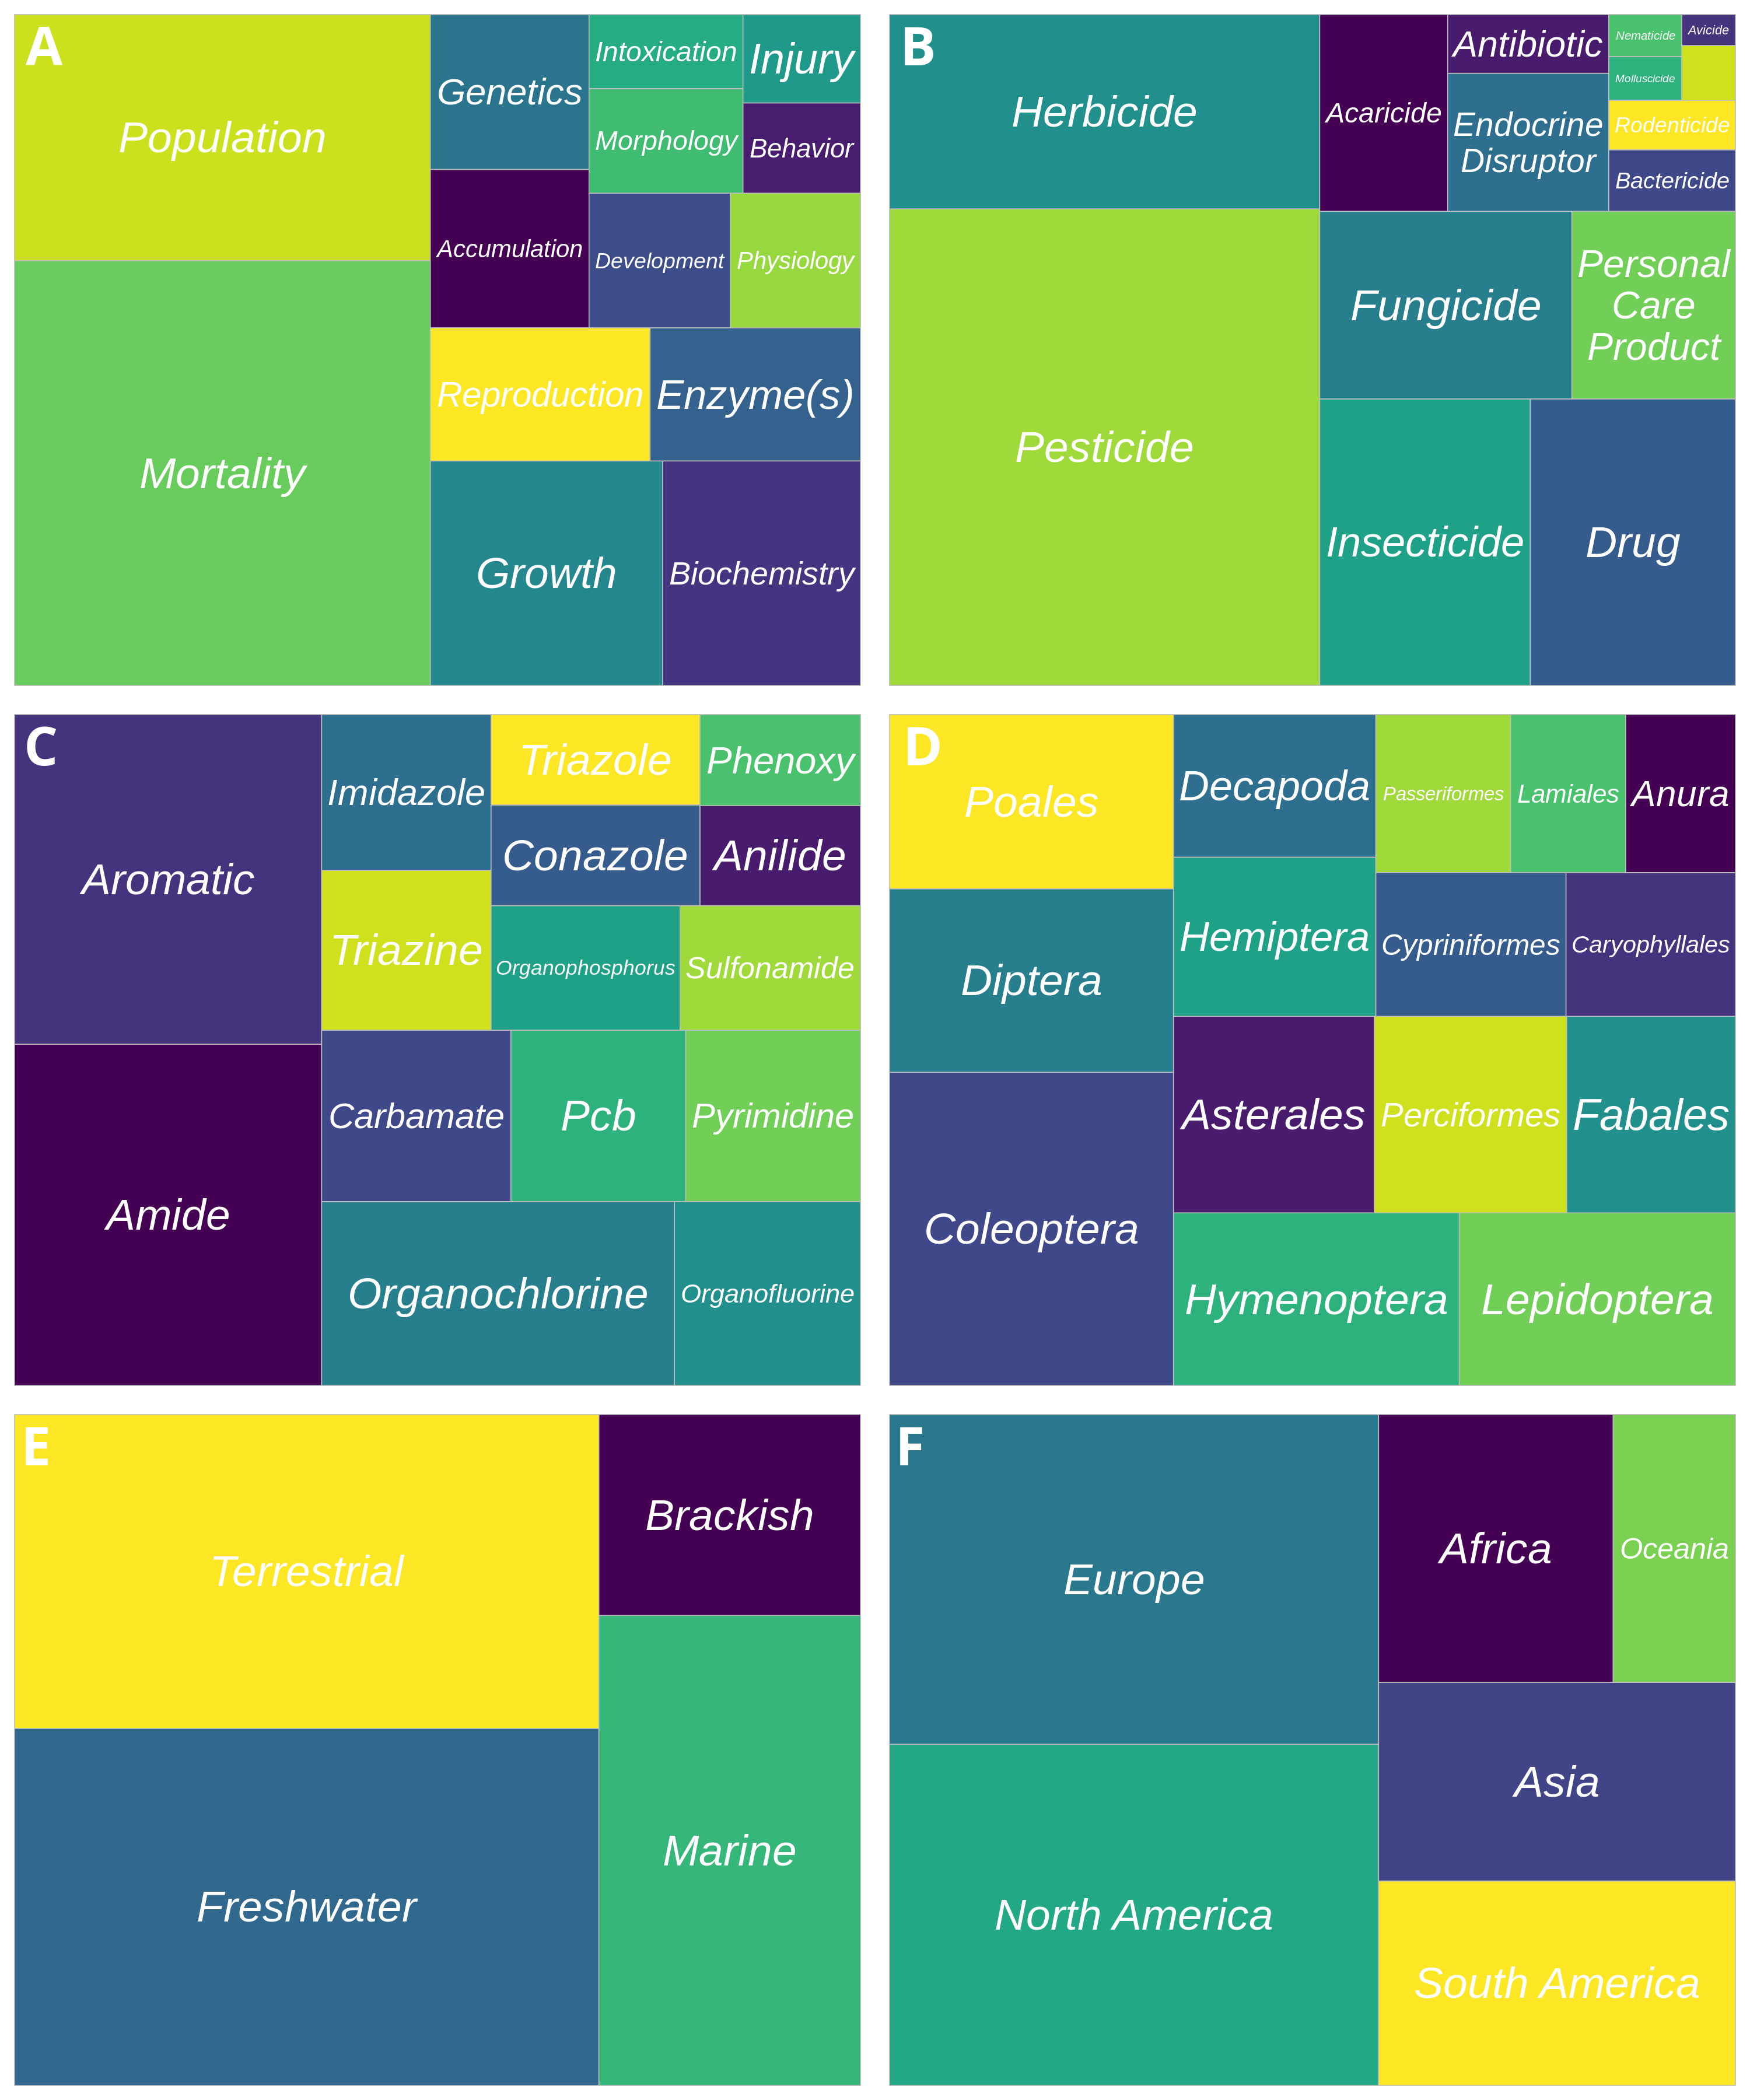
\includegraphics[width=0.55\textwidth]{figures/standartox_parameters.png}
    \caption{Share of 10 most frequent entries for the parameters (\textbf{A}) effect group, (\textbf{B}) chemical role, (\textbf{C})~chemical class, (\textbf{D}) taxonomic order, (\textbf{E}) organism habitat and (\textbf{F}) organism distribution in Standartox. Multiple classifications are possible (e.g. a chemical can be a fungicide and a pesticide).}
    \label{fig:stx-parameters}
\end{figure}
\unskip

\subsection{Aggregation}
Typically, species exhibit a differential sensitivity towards chemicals (Figure~\ref{fig:stx-variability}A). Moreover, multiple ecotoxicity values are available for individual species-chemical combinations and these can also exhibit high variability due to several factors such as durations of ecotoxicity tests (Figure~\ref{fig:stx-variability}B), experimental conditions and physiological or genetic fitness differences between test individuals or populations. Not every factor is recorded though, leading to unexplainable variability (Figure~\ref{fig:stx-variability}C). To~aggregate multiple ecotoxicity values into a single value on the desired taxonomic level (e.g., for an individual species, across species of a genus or family), and~chemical grouping (e.g., across all pesticides), Standartox provides several aggregation methods including the minimum, the~maximum and the geometric mean allowing to aggregate the filtered data set. The~geometric mean is preferred in comparison to the arithmetic mean, because~it is less influenced by outliers and is suitable for skewed data. Furthermore, the~geometric mean is preferable over the median, because~the median completely ignores the tails of the data distribution, making it unreliable for small data sets~\citep{leith_comparison_2010}. \citet{posthuma_species_2019} showed the usefulness of SSDs and its underlying geometric mean aggregations when assessing environmental effects of chemicals. In~the course of the aggregation process, outliers that exceed 1.5 times the interquartile range are flagged to caution Standartox users. However, they are considered in the aggregation, given that the geometric mean is relatively robust against outliers. Overall, Standartox provides a harmonized and reproducible approach to aggregate ecotoxicity data.

\begin{figure}[H]
    \centering
    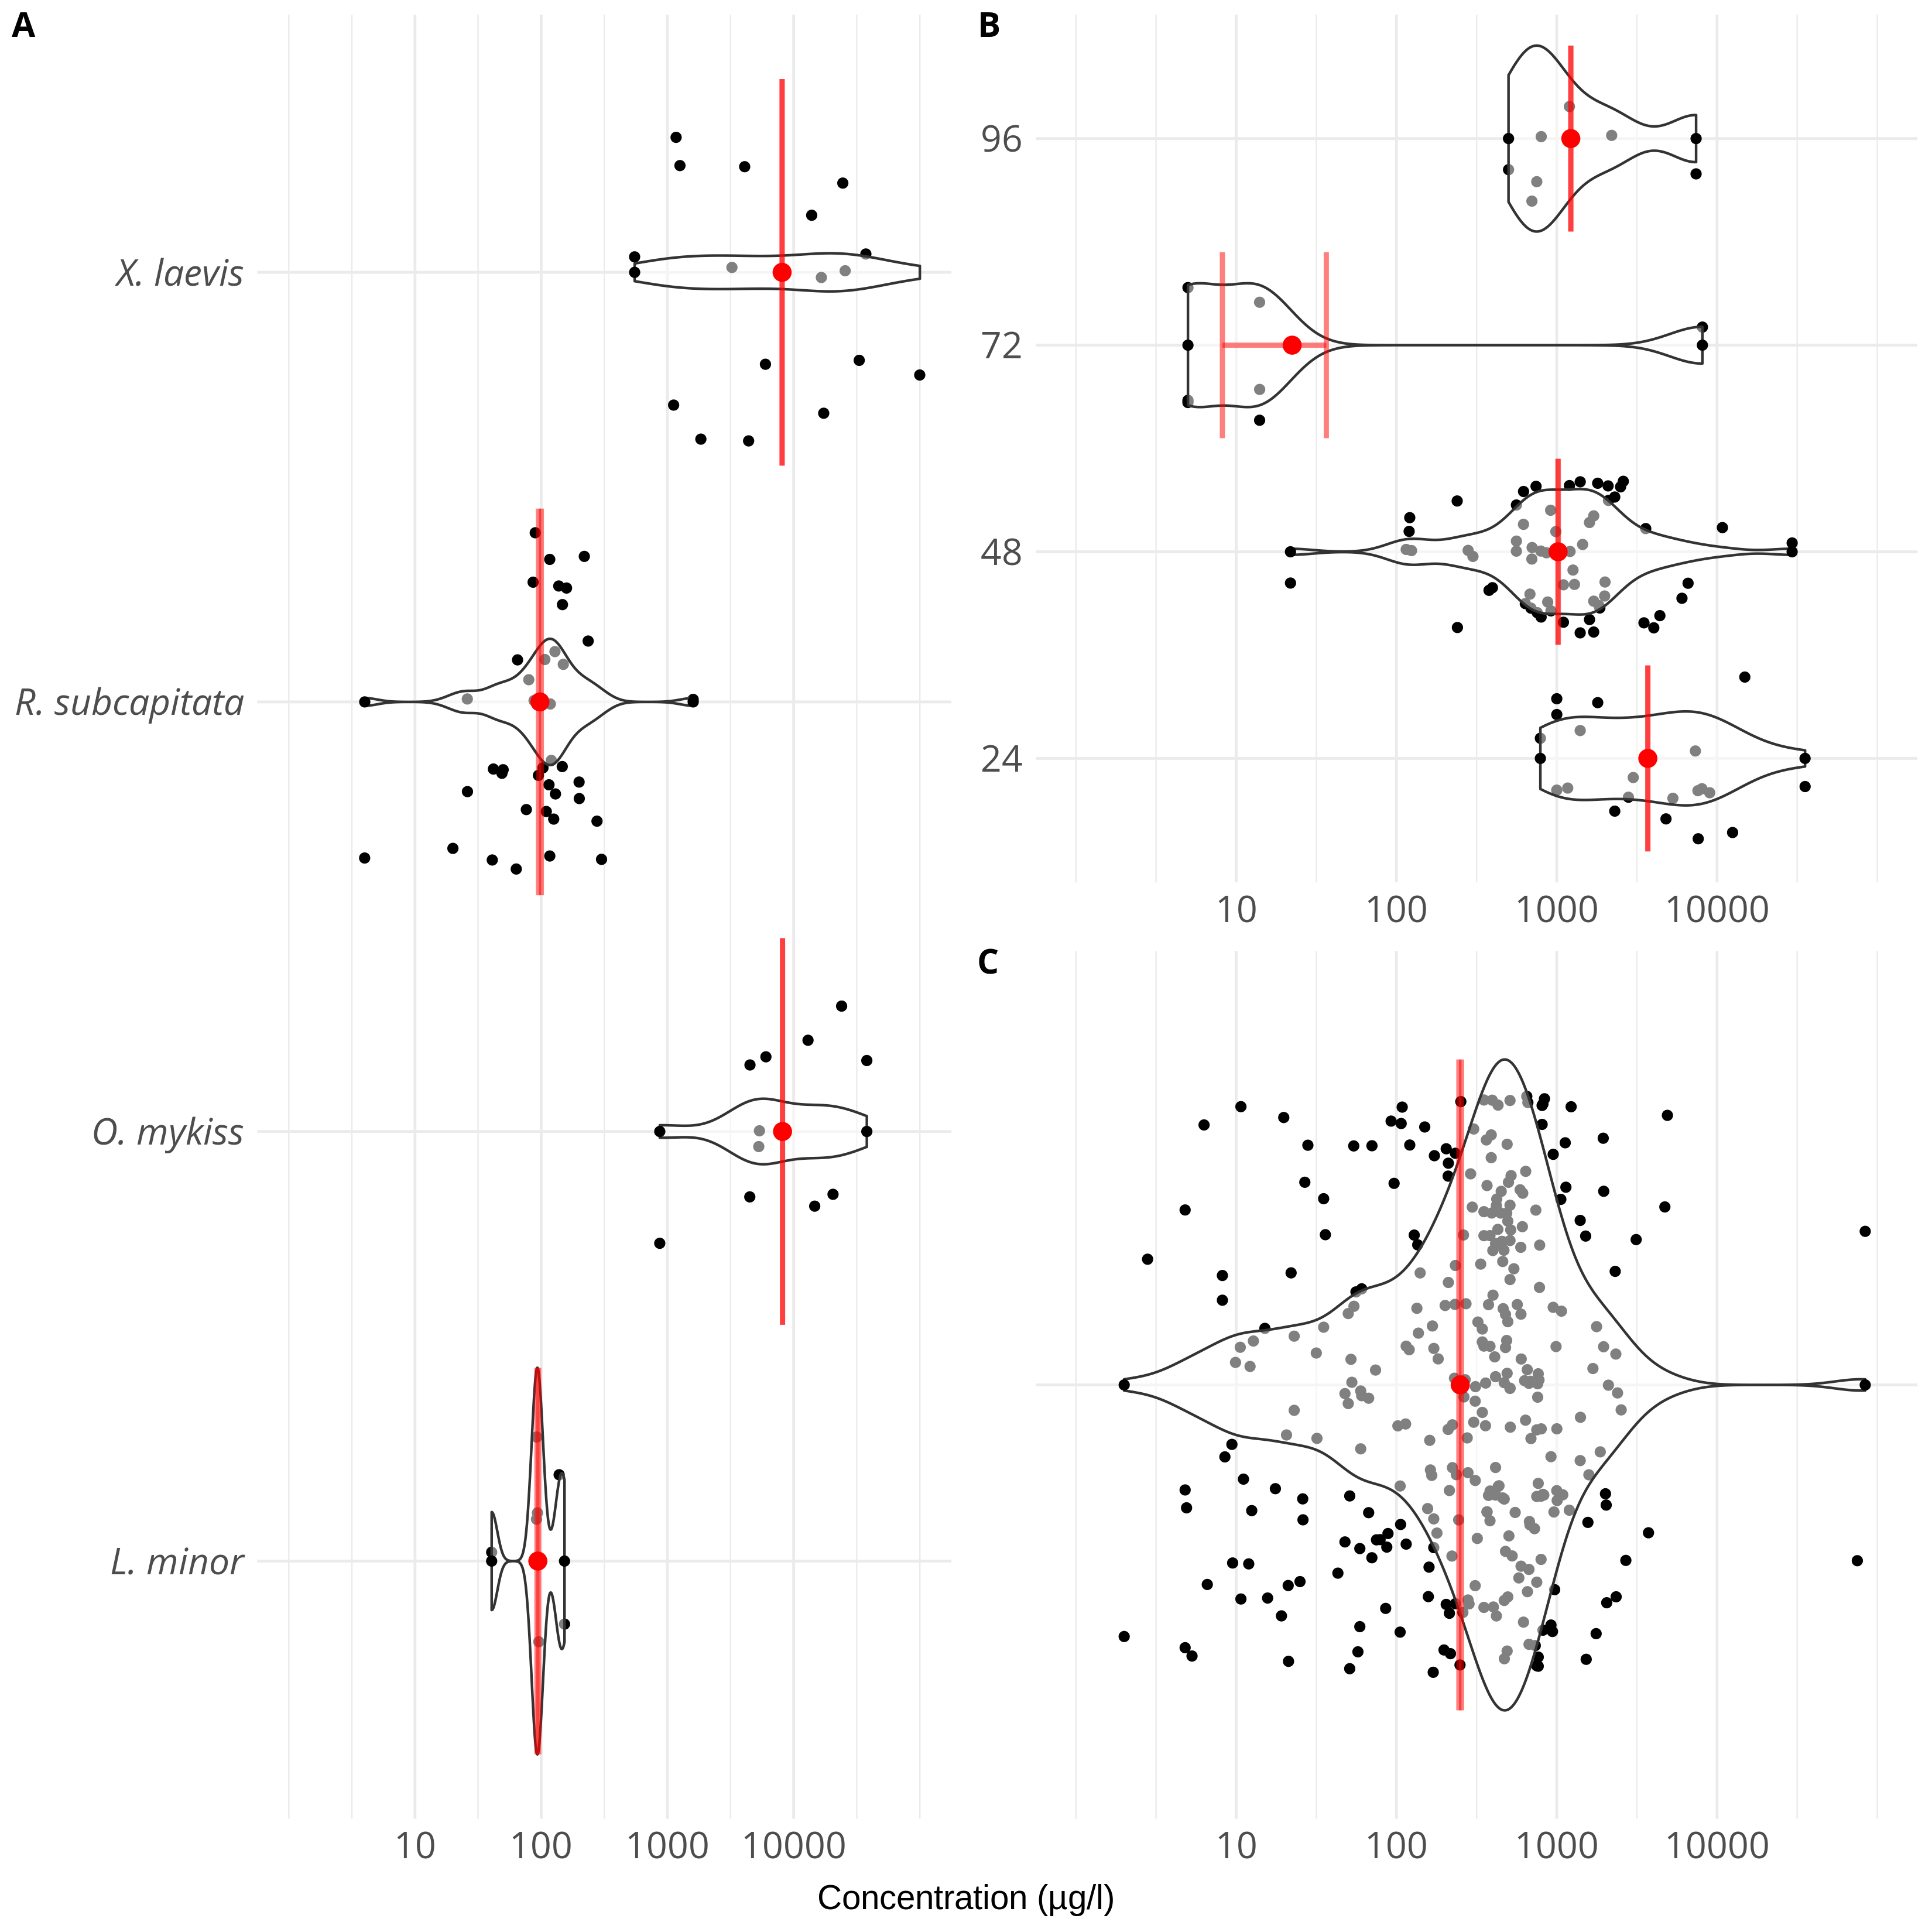
\includegraphics[width=0.65\textwidth]{figures/results_variability.png}
    \caption{Violin plots of of test results (XX\textsubscript{50}) in Standartox illustrating (\textbf{A}) differential variability and data distribution between species (i.e., \textit{Xenopus laevis}---Amphibian, \textit{Raphidocelis subcapitata}---Algae, \textit{Oncorhynchus mykiss}---Fish, \textit{Lemna minor}---Macrophyte) for the chemical atrazine in 96 h tests, (\textbf{B}) how the variability in toxicity tests with zinc sulfate and \textit{Daphnia magna} varies with test duration and (\textbf{C})~high variability that is not explained by the available test characteristics in the case of cupric sulfate tested on \textit{Pimephales promelas} for 96 h. Red dots depict Standartox geometric mean estimates and red error bars show the associated standard deviation. Black dots depict the raw data. To~facilitate readability, data points are randomly scattered along a hypothetical y-axis and are greyed out if within the~violins.}
    \label{fig:stx-variability}
\end{figure}
\unskip

\subsection{Accuracy~Assessment}
To validate Standartox results we compared geometric means resulting from the aggregation in Standartox to the corresponding values from other databases, for~chemicals where data were available in both resources. The~PPDB provides ecotoxicity data on a few selected species commonly used in chemical risk assessment, that have been manually quality controlled through expert judgment~\citep{lewis_international_2016}. The~vast majority of aggregated values (91.9~\%) of Standartox lie within one order of magnitude of the corresponding PPDB values (n~=~3601). This would increase to 92.6~\%, when restricting the comparison to Standartox values where data from at least five experiments are available. Similarly, we compared Standartox to ecotoxicity values for \textit{Daphnia magna} from the ChemProp~\citep{ufzdepartmentofecologicalchemistry_chemprop_2016} software, which estimates LC\textsubscript{50} values via quantitative structure-activity relationship (QSAR) models~\citep{schuurmann_quantitative_2011}. We found that 95~\% of Standartox values lie within one order of magnitude of the ChemProp (n~=~179) values. However, the~difference is not necessarily an indication of lower quality of Standartox estimates but may also reflect the wider range of experimental conditions for which data are available in the database underlying Standartox as well as inaccurate predictions for QSAR models, respectively (Figure~\ref{fig:standartox_ppdb_diff}).

\begin{figure}[H]
    \centering
    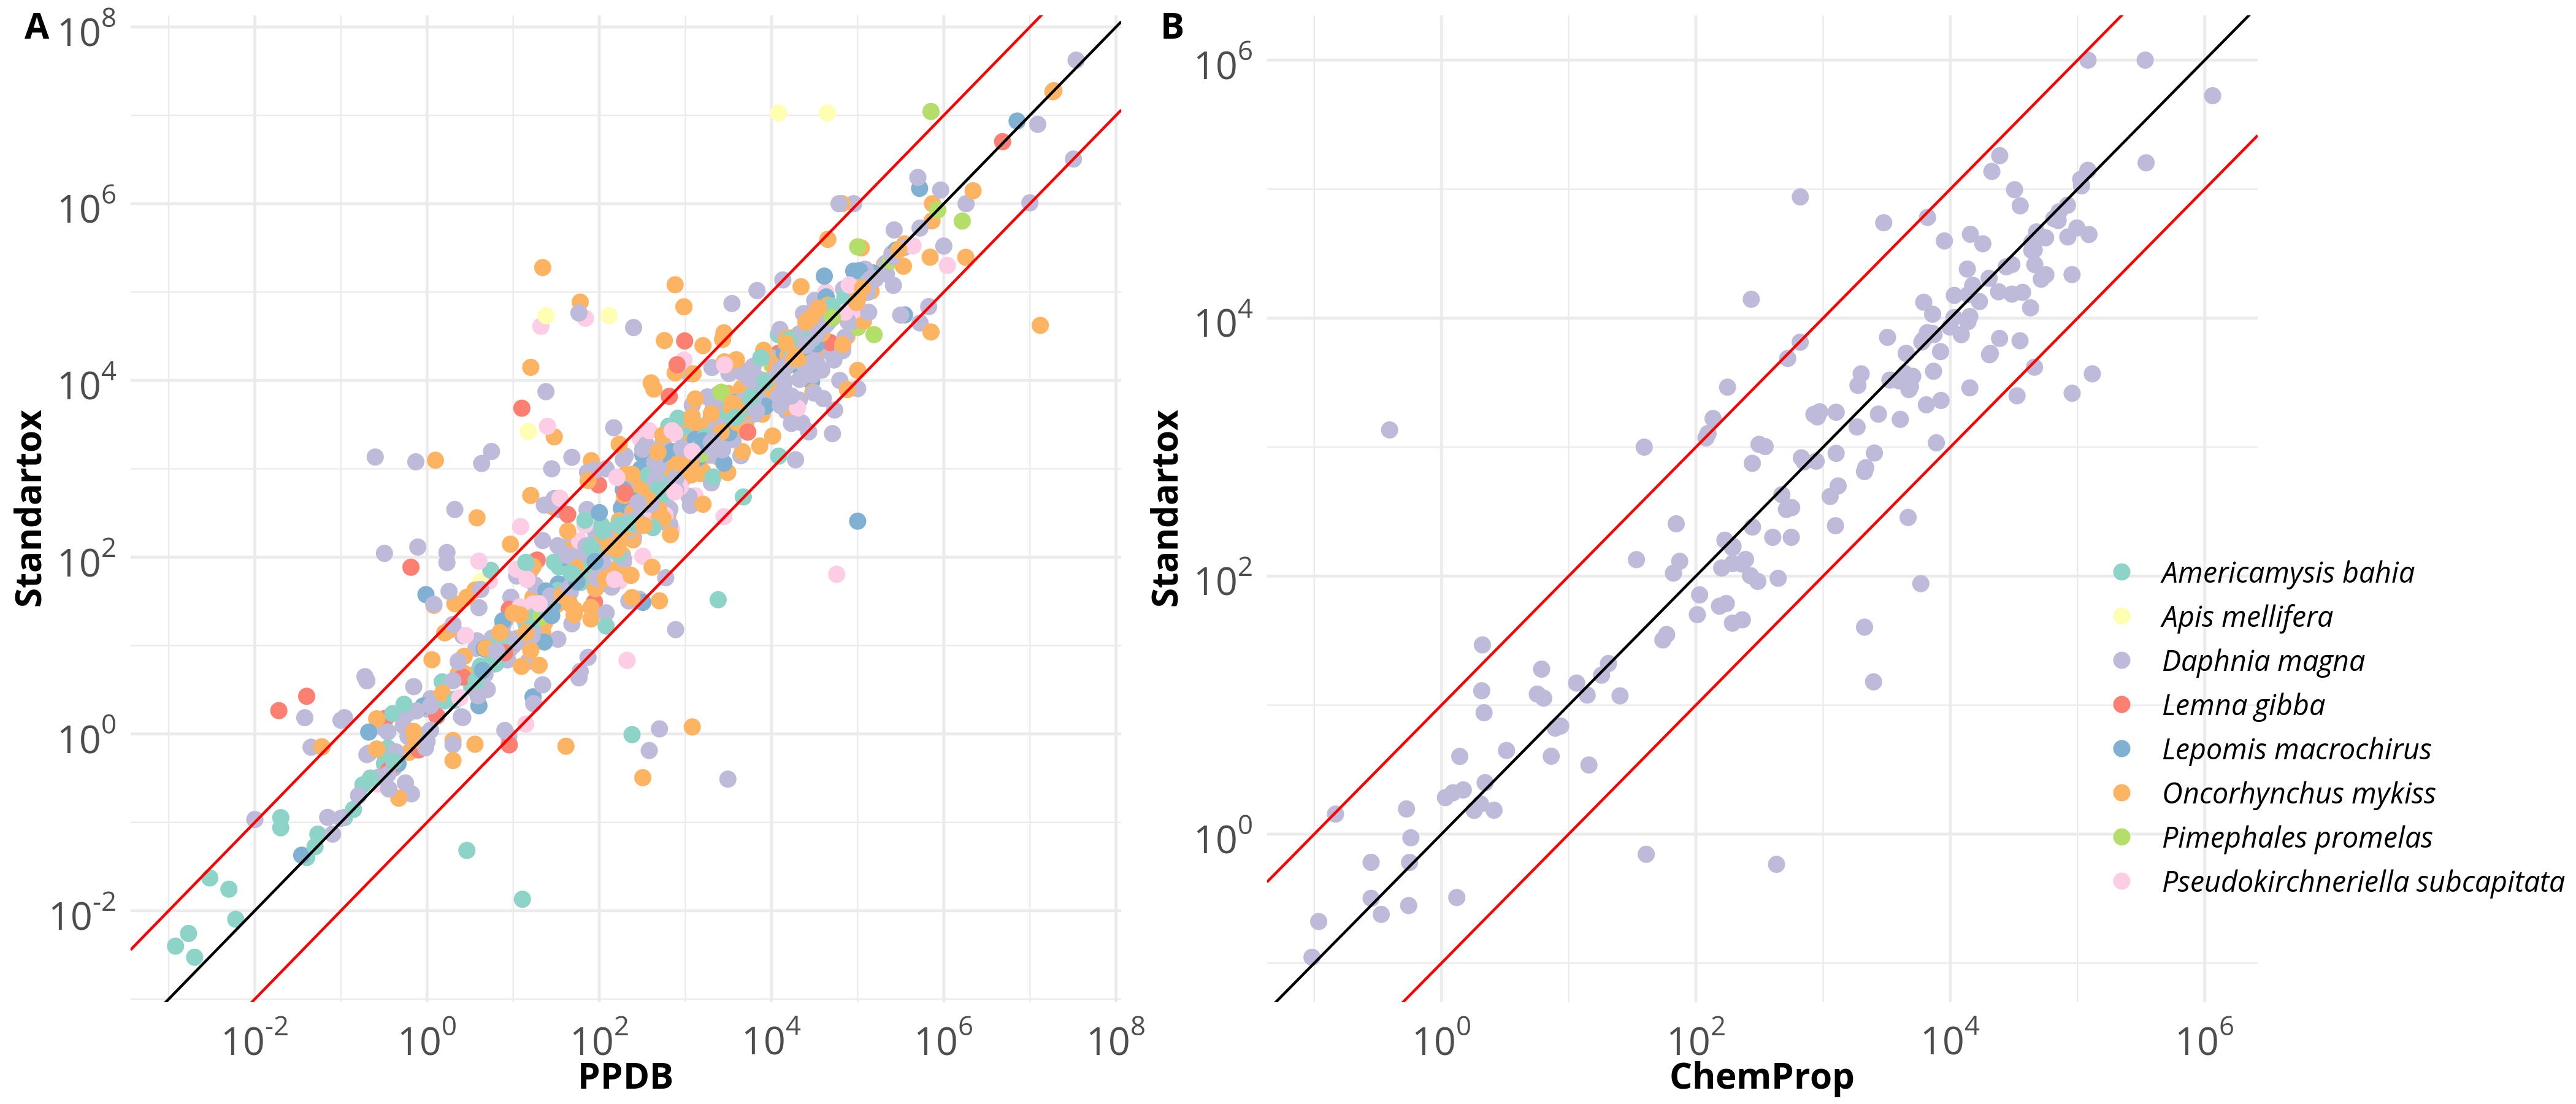
\includegraphics[width=.98\linewidth]{figures/gg_ppdb_stan_compare_continous.png}
    \caption{Comparison between Standartox, (\textbf{A}) the Pesticides Properties DataBase (PPDB) %define; %AS done
        and (\textbf{B}) ChemProp values. The~black lines indicate identity and red lines mark a divergence of a factor of 10. Compared species are color~coded.}
    \label{fig:standartox_ppdb_diff}
\end{figure}
\unskip

\subsection{Perspectives}
Novel predictive frameworks incorporating chemical mode of action and species traits emphasize the need for holistic and automated analyses of large-scale ecotoxicological data~\citep{malaj_evolutionary_2016, vandenberg_modeling_2019}. Indeed, the~increasing amount of data from ecotoxicological tests and experiments that is becoming available has elicited several initiatives to harmonize these data. These initiatives partly aim for overlapping goals, yet have limitations or objectives that distinguish them from Standartox:
\par
\textbf{Comptox}, is a web tool published by the EPA which, similar to Standartox allows for filtering test results, the~retrieval of additional chemical information as well as predicted toxicity data~\citep{martin_prediction_2001}, such as 48 h \textit{Daphnia magna} LC\textsubscript{50} values. However, toxicity estimations are limited to standard test organisms, and~the tool lacks the possibility for automated data retrieval~\citep{williams_comptox_2017}. \textbf{Comptox} is built on the Aggregated Computational Toxicology Resource (\textbf{ACToR}) database, which constitutes the basis for several applications published by the EPA. It collects physicochemical and toxicological data on more than 500,000 environmental chemicals and pharmaceutical compounds from various resources and presents them in a curated list on the web~\citep{judson_actor_2008, judson_aggregating_2012}. However, no filter mechanisms or aggregation methods are provided in ACToR per se.
\par
The \textbf{EnviroTox} database which also uses, amongst others the ECOTOX database as an input has recently been published~\citep{healthandenvironmentalsciencesinstitutehesi_envirotox_2019, connors_creation_2019}. In~contrast to Standartox, EnviroTox  is restricted to selected aquatic organisms (i.e., fish, amphibians, invertebrates and algae) and experimental durations (at~least 24~h) and uses a rule-based algorithm to derive single ecotoxicity values. Besides, EnviroTox provides additional information on toxicity endpoints, such as acute or chronic classifications and mode of action assignments. We intentionally omitted such classifications given that the approach to classification may vary with the purpose of the study or because of different classification schemes~\citep{kienzler_mode_2017}. The~EnviroTox database allows for an aggregation into single toxicity values for individual taxa, whereas Standartox performs this aggregation for individual chemical-taxa combinations. However, the~Standartox results for individual taxa-chemical combinations could easily be aggregated across chemicals in a second step to provide a similar aggregation as that performed in EnviroTox.
\par
The \textbf{Etox} database collects ecotoxicity test information and provides methods to filter those. Like the ECOTOX database, it also lacks methods to perform aggregations of the ecotoxicity data and only provides manual (non-automated) access. In~contrast to the latter, the~Etox database can not be downloaded as a whole.
\par
The \textbf{PPDB} provides data only on pesticides, and~as mentioned before, it provides single quality controlled values only for commonly used taxa, e.g.,~\textit{Daphnia magna} or \textit{Raphidocelis subcapitata}.
\par
In summary, none of the above mentioned initiatives aim for an automated and standardized aggregation method of exposure endpoints for individual chemicals. In~addition, they lack the possibility to access the databases through a common high level programming language, such as~R. An overview of the filter and aggregation methods as well as the accessibility of the presented databases is presented in Table \ref{tab:database-differences}.

\begin{table}[H]
    \caption{\textls[-15]{\hl{Overview on databases that provide ecotoxicological data.} Abbreviations: ALL: Most important test parameters, including chemical, taxon, duration for filtering ecotoxicological data are incorporated.} Web: Accessible via a web application through a graphical user interface. API: Accessible via an application programming~interface.} %This table has not been referred to within the text of the manuscript.; %AS done

    \label{tab:database-differences}
    \centering
    \begin{tabular}{ccccc}
    \toprule
    \textbf{Database} & \textbf{Filter} & \textbf{Aggregation, Selection} & \textbf{Access} \\
    \midrule
    Comptox~\citep{williams_comptox_2017} & Chemical & no & Web, file \\
    Ecotox~\citep{usepa_ecotox_2019} & ALL & no & Web, file \\
    EnviroTox~\citep{healthandenvironmentalsciencesinstitutehesi_envirotox_2019} & ALL & chemical, organism & Web \\
    Etox~\citep{umweltbundesamt_etox_2019} & ALL & no & Web \\
    Pesticides Properties DataBase (PPDB)~\citep{lewis_international_2016} & fixed values & manual selection & Web, file \\
    Standartox & ALL & chemical, organism & API, Web \\
    \bottomrule
\end{tabular}
\end{table}

\par
As outlined above, toxicity estimates from different studies can vary strongly due to a wide range of experimental conditions such as pH, temperature and conductivity~\citep{rosenkrantz_influence_2013, li_temperature_2011}. Integrating these conditions into the aggregated estimates would certainly improve toxicity estimates. However, the~current implementation of Standartox omits these conditions, because~the ECOTOX database only provides sparse records on experimental conditions. The~most frequently provided experimental conditions are temperature (77\%), pH (56\%), hardness (27\%), dissolved oxygen (18\%), Alkalinity (15\%) and salinity (9\%). For~all other conditions less than 5\% of data entries are available. A~text-mining approach, where a literature reference is associated with ecotoxicity raw data, iterating through the individual publications could potentially increase this number, e.g.,~\citet{compson_linking_2018} successfully applied text-mining techniques to retrieve species trait~data. 

%%%%%%%%%%%%%%%%%%%%%%%%%%%%%%%%%%%%%%%%%%
\section{Methods}
An automated processing pipeline downloads the quarterly released ECOTOX database, performs several preparation steps on it and exports a final Standartox data set. This data set is accessible via a web application and an application programming interface (API). An~API provides the means for machine communication between a host and a client and thus allows scriptable data queries. To~facilitate the API access, the~R~\citep{rcoreteam_language_2020} package \textit{standartox} is built. All data presented in this paper are derived from the Standartox build, based on the ECOTOX release from the 12.12.2019. The~code for Standartox is located in the two Github repositories \textit{andschar/standartox-build}~\footnote{\url{https://github.com/andschar/standartox-build}} and \textit{andschar/standartox}~\footnote{\url{https://github.com/andschar/standartox}}. The~former contains code to process the data and to build the web application and the API, the~latter contains code to build the R~package. Most of the code is written in R 3.6.1 and associated packages (List: Table~\ref{tab:rpackages}) and in Structured Query Language (SQL) for PostgreSQL~9.6.1. A graphical overview of the most important processing steps is given in Figure \ref{fig:stx-organigram}. %please correct the reference citation; %AS done

\subsection{Processing}
Standartox downloads the quarterly released ECOTOX database and builds it into a local PostgreSQL database. Subsequently, SQL functions for further processing the data are implemented. In~addition lookup tables that enable the conversion of units such as duration and concentration are created. A~meta-table providing information, such as the release version of the ECOTOX database is added. Then, provided Chemical Abstracts Service (CAS) numbers and taxonomic names are used to query additional information from publicly available databases on chemicals and organisms, respectively. This includes the Compendium of Pesticide Common Names~\citep{wood_compendium_2019}, the~Chemical Entities of Biological Interest (ChEBI) database~\citep{hastings_chebi_2016}, the~Chemical Identifier Resolver (CIR) service~\citep{nationalinstitutesofhealthnih_chemical_2019}, the~Pubchem database~\citep{kim_pubchem_2016}, Eurostat~\citep{europeancommission_eurostat_2019} and Wikidata~\citep{vrandecic_wikidata_2014} for chemicals and the World Register of Marine Species (WoRMS)~\citep{wormseditorialboard_world_2020}, the~Global Biodiversity Information Facility (GBIF)~\citep{gbiftheglobalbiodiversityinformationfacility_what_2020} and the freshwaterecology.info database~\citep{schmidt-kloiber_www_2015} for habitat and spatial distribution of organisms (Table~\ref{tab:data-base-additional}). Given that taxonomic names can be ambiguous, e.g.,~the genus \textit{Eisenia} can refer to an algae and a worm, we first match the taxa names against specific database identifiers and subsequently check their accordance with the underlying ECOTOX data taxonomy. Then, we query the actual data by using the identifiers. In~a next step, the data are added to Standartox to enable filtering for specific chemical roles (e.g., drug, metal, pesticide, personal care product) and classes (e.g., pyrethroid, carbamate) as well as spatial distribution (i.e., continents) and habitat preferences (e.g., freshwater) of individual taxa. Taxa that were not identified to at least genus level are excluded, because~relative toxicity comparisons have been shown to be not meaningful for higher taxonomic levels~\citep{rainbow_trace_2002, buchwalter_differences_2005, malaj_physiological_2012}. Finally, the~Standartox data set is compiled, which includes the harmonisation of data, e.g.,~through conversion of test concentration and duration units. 1237 distinct concentration units are converted to six harmonized ones (i.e., g/L, g/m\textsuperscript{2}, ppb, g/g, L/L and L/m\textsuperscript{2}) when conversion is possible. Likewise, the~126 distinct duration units are converted to hours whenever this is unambiguously possible. To~guarantee appropriate unit conversion and harmonisation, we compared the results of an automated unit conversion to a manual one for each of the distinct concentration and duration units. This assures that 652 of the 1237 concentration units (95.3\% of the data) are converted correctly. The~remainder could not be converted and is removed.  Furthermore, the~units are cleaned, for~example through removing additional information in the field such as \textit{food}, \textit{soil}, \textit{ai} that are also coded in other variables and hinder the processing of units. Concentrations that are given as rates such as per day (e.g., mg/kg/day) are multiplied by the days of the test and then converted. Experimental endpoints are restricted to three groups, namely NOEX, LOEX and XX\textsubscript{50}. Other endpoints, such as Bioconcentration factors, non-half maximal effective concentrations (e.g., IC\textsubscript{10}, EC\textsubscript{25}, LD\textsubscript{99}) or maximum acceptable toxicant concentrations are removed. Along with that, a~catalog, listing all distinct entries and value ranges, for~categorical and continuous variables, respectively, is created. The~compiled Standartox data set together with the catalog is exported and accessible via the web application and the API, through the R~package.

\begin{figure}[H]
    \centering
    \includegraphics[scale=0.75]{figures/fig4.png}
    \caption{\hl{Organigram of Standartox.} The U.S. Environmental Protection Agency (EPA) ECOTOXicology Knowledgebase (ECOTOX) is downloaded quarterly and processed (i.e., query additional information with Chemical Abstracts Service (CAS) numbers 
    and taxa names and conversion of concentration and duration units). Subsequently, a~Standartox data set is compiled together with filter and aggregation methods. Thus, users can access the Standartox data set and filter and aggregate through a web application and an~R~package.} %This figure has not been referred to within the text of the manuscript.

    \label{fig:stx-organigram}
\end{figure}
\unskip

\subsection{Application~Methods}
\textls[-15]{When accessed, the~web application and the API load the compressed serialized Standartox data into memory and allows the user to interact with them.} The~user can then call the functions \textit{stx\_filter()} and \textit{stx\_aggregate()} that filter and aggregate the data according to specific parameters (Table~\ref{tab:app-parameters}). The~interactive web application is built in R using the shiny framework, which runs with the help of a shiny {server}~\citep{R-shiny}. The~API is built by using the R~package {\textit{plumber}}~\citep{R-plumber}, which allows for the creation of Representational State Transfer (REST) APIs from R. REST is a software architectural style that defines web service communication rules. The~API is reachable via the Internet Protocol (IP) address 139.14.20.252 and port 8000. Three API-endpoints (\textit{/catalog}, \textit{/filter}, and~\textit{/meta}) can be queried (Table~\ref{tab:api-endpoints}). The~\textit{/catalog} API-endpoint returns a JavaScript Object Notation (JSON) file containing a catalog of possible filter parameters to choose from. The~\textit{/filter} returns the filtered Standartox table as a compressed serialized binary file created by the R~{package}~\textit{fst}~\citep{R-fst}, to~reduce size and allow for fast user queries. Lastly, the~\textit{/meta} API-endpoint returns a JSON file with meta information, such as the timestamp of the request and the used Standartox version. The~API is designed to be used with the R~package \textit{standartox} and therefore uses serialization methods specific to R (rds() from the R~package \textit{base} and fst() from the R~package \textit{fst}). To~facilitate the API usage the R~package \textit{standartox} is~created.%please correct the reference citation

\begin{table}[H]
    \caption{Input parameters for the Standartox web application and the R package \textit{standartox} (CAS---Chemical Abstracts Service Registry number, NOEX and XX\textsubscript{50}---Standartox endpoints Table~\ref{tab:endpoints-conflate}), vers---Standartox version).}
    \label{tab:app-parameters}
    \centering
    \begin{tabular}{cc}
    \toprule
    \textbf{Parameter} & \textbf{Example} \\ 
    \midrule
    cas & 7758987, 2921-88-2, 1912-24-9 \\
    concentration\_type & Active ingredient, Formulation \\
    chemical\_role & Antibiotic, Fungicide, Drug \\
    chemical\_class & Conazole, Neonicotinoid, Triazine \\
    taxa & Oncorhynchus mykiss, Rattus norvegicus, Daphnia magna \\
    habitat & Marine, Brackish, Freshwater \\
    region & Europe, Africa, Asia \\
    duration & 24, 96 \\
    effect & Mortality, Population, Growth \\
    endpoint & NOEX, XX50 \\
    exposure & auquatic, diet \\
    vers & 20191212 \\
    \bottomrule
\end{tabular}
\end{table}
\unskip

%%%%%%%%%%%%%%%%%%%%%%%%%%%%%%%%%%%%%%%%%%
\section{User~Notes}
Users can access Standartox either via the web application~\footnote{\url{http://standartox.uni-landau.de}} or via the R~package \textit{standartox}. By~accessing the web application, users can filter and download the resulting data sets as a comma-separated values (csv) file. Users of the R~package can directly load the data within R. The~R~package provides the two functions \textit{stx\_catalog()} and \textit{stx\_query()}. The~first command queries a catalog of possible Standartox parameters into an R list object. The~latter allows users to set the Standartox filter parameters and to fetch the actual data. It returns an R list of three tables (i.e., R \textit{data.frame}s) containing the filtered data set, the~aggregated data set and a table with the meta information retrieved from the API endpoints. A~short R-code example is given below (Listing \ref{lis:standartox-example}) and a detailed description on the usage of the R~package is provided on its Github page~\footnote{\url{https://github.com/andschar/standartox}}.

\begin{lstlisting}[
    language = R,
    caption = {Sample code to access the Standartox database through the API and the the R package \textit{standartox}. \textit{stx\_catalog()} returns a catalog of possible filter and aggregation parameters. \textit{stx\_query()} returns the Standartox object, a~list of the filtered and the aggregated data as well as a meta data entry. Example for XX\textsubscript{50} tests on the chemical glyphosate (CAS number: 1071-83-6) and the taxon \textit{Oncorhynchus} lasting 24 h to 120 h.},
    label = {lis:standartox-example}]
# install
install.packages('remotes')
remotes::install_github('andschar/standartox')
# retrieve catalog    
require(standartox)
catal = stx_catalog()
# retrieve data
l = stx_query(cas = '1071-83-6',
              endpoint = 'XX50',
              taxa = 'Oncorhynchus',
              duration = c(24, 120))
\end{lstlisting}
\newpage
%%%%%%%%%%%%%%%%%%%%%%%%%%%%%%%%%%%%%%%%%%
\section{Conclusions}
% This section is not mandatory, but can be added to the manuscript if the discussion is unusually long or complex.
Due to the steady incorporation of new ecotoxicity data, the~aggregated values produced by Standartox can be subject to change with future updates. We regard this as an advantage rather than a drawback because other published works that aim in a similar direction often constitute a singular effort or require manual work for each update. Standartox, in~contrast, automates the update process, yet still provides access to its older versions, assuring reproducibility and version control. In~comparison to rule-based approaches for the derivation of single ecotoxicity values, Standartox has the advantage to be free from the subjectivity of a set of human-induced rules. Above~all, Standartox provides quick access through its design to be queried via the R language. Due to an increased amount of available ecotoxicological test data, it becomes fundamental to provide and distribute ecotoxicity information in adequate formats, both easily accessible for humans and easily processable for machines. Standartox meets these requirements and puts its focus on the aggregation of toxicity data, thereby adding a piece to the puzzle of modern ecotoxicological data analyses.

%%%%%%%%%%%%%%%%%%%%%%%%%%%%%%%%%%%%%%%%%%
\vspace{6pt} 

%%%%%%%%%%%%%%%%%%%%%%%%%%%%%%%%%%%%%%%%%%
%% optional
%\supplementary{The following are available online at \linksupplementary{s1}, Figure S1: title, Table S1: title, Video S1: title.}

% Only for the journal Methods and Protocols:
% If you wish to submit a video article, please do so with any other supplementary material.
% \supplementary{The following are available at \linksupplementary{s1}, Figure S1: title, Table S1: title, Video S1: title. A supporting video article is available at doi: link.}

%%%%%%%%%%%%%%%%%%%%%%%%%%%%%%%%%%%%%%%%%%
\authorcontributions{Conceptualization and methods, A.S., R.B.S. and V.C.S.; software development and validation, A.S.; data curation and analysis, A.S.; writing--original draft preparation, A.S.; writing--review and editing, A.S., V.C.S. and R.B.S.; supervision, R.B.S. All authors have read and agreed to the published version of the manuscript.}
% \authorcontributions{conceptualization, A.S., R.B.S. and V.C.S.; methodology, A.S.; software, A.S.; validation, A.S., Y.Y. and Z.Z.; formal analysis, X.X.; investigation, X.X.; resources, X.X.; data curation, X.X.; writing--original draft preparation, X.X.; writing--review and editing, X.X.; visualization, X.X.; supervision, X.X.; project administration, X.X.; funding acquisition, Y.Y.''}

%%%%%%%%%%%%%%%%%%%%%%%%%%%%%%%%%%%%%%%%%%
\funding{This research was funded by the German Environment Agency (UBA) grant number 3714 67 4040/2.}

%%%%%%%%%%%%%%%%%%%%%%%%%%%%%%%%%%%%%%%%%%
\acknowledgments{The authors thank Eduard Szöcs for inspiration through a blog post on how to build a local version of the EPA ECOTOX~database.}

%%%%%%%%%%%%%%%%%%%%%%%%%%%%%%%%%%%%%%%%%%
\conflictsofinterest{The authors declare no conflict of~interest.} 
%%%%%%%%%%%%%%%%%%%%%%%%%%%%%%%%%%%%%%%%%%
\abbreviations{The following abbreviations are used in this manuscript:\\

\noindent 
\begin{tabular}{@{}ll}
API & Application programming interface \\
CAS & Chemical abstracts service registry number \\
ChEBI & Chemical Entities of Biological Interest database \\
CIR & Chemical Identifier Resolver service \\
E/LC/D\textsubscript{50} &  Half maximal effective/lethal concentration/dose \\
XX\textsubscript{50} & Summarizes E/LC/D\textsubscript{50} (Table \ref{tab:endpoints-conflate}) \\
ECOTOX & US EPA ECOTOXicology Knowledgebase \\
GBIF & Global Biodiversity Information Facility \\
JSON & JavaScript Object Notation file format \\
LOEC/L & Lowest observed effect concentrations/levels \\
LOEX & Summarizes LOEC/L (Table \ref{tab:endpoints-conflate}) \\
NOEC/L & No observed effect concentrations/levels \\
NOEX & Summarizes NOEC/L (Table \ref{tab:endpoints-conflate}) \\
PPDB & Pesticides Properties DataBase \\
QSAR & Quantitative structure-activity relationship \\
REST & Representational state transfer software architectural style \\
SSD & Species sensitivity distribution \\
TU & Toxic unit \\
WoRMS & World Register of Marine Species \\
\end{tabular}
}

%%%%%%%%%%%%%%%%%%%%%%%%%%%%%%%%%%%%%%%%%%
%% optional
\appendixtitles{no} %Leave argument "no" if all appendix headings stay EMPTY (then no dot is printed after "Appendix A"). If~the appendix sections contain a heading then change the argument to "yes".
\appendix
\section{}
\begin{table}[H]
    \caption{Table of additionally queried publicly available databases and their~URLs.}
    \label{tab:data-base-additional}
    \centering
\begin{tabular}{cc}
    \toprule
    \textbf{Database} & \textbf{URL} \\ 
    \midrule
    \makecell{Chemical Entities of \\ Biological Interest (ChEBI)} & \url{https://www.ebi.ac.uk/chebi} \\
    Chemical Identifier Resolver & \url{https://cactus.nci.nih.gov/chemical/structure} \\[0.5cm]
    ChemSpider & \url{http://www.chemspider.com}    \\[0.5cm]
    Eurostat & \url{https://ec.europa.eu/eurostat/home} \\[0.5cm]
    PubChem & \url{https://pubchem.ncbi.nlm.nih.gov} \\[0.5cm]
    Wikidata & \url{https://www.wikidata.org/wiki/Wikidata:Main_Page} \\[0.5cm]
    \makecell{Global Biodiversity \\ Information Facility (GBIF)} & \url{https://www.gbif.org} \\[0.5cm]
    \makecell{World Register of \\ Marine Species (WoRMS)} & \url{http://marinespecies.org} \\
    \makecell{freshwaterecology.info} & \url{https://www.freshwaterecology.info} \\
    \bottomrule
\end{tabular}
\end{table}
\unskip

\begin{table}[H]
    \caption{Table of how Standartox endpoints are derived from EPA ECOTOX~endpoints.}
    \label{tab:endpoints-conflate}
    \centering
\begin{tabular}{ccc}
    \toprule
    \textbf{Standartox Endpoint} & \textbf{Ecotox Endpoint} & \textbf{Ecotox Endpoint Description} \\
    \midrule
    XX\textsubscript{50} & LC\textsubscript{50} & Lethal concentration to 50\% of test organisms \\
    XX\textsubscript{50} & LD\textsubscript{50} & Lethal dose to 50\% of test organisms \\
    XX\textsubscript{50} & EC\textsubscript{50} & Effective concentration to 50\% of test organisms \\
    XX\textsubscript{50} & ED\textsubscript{50} & Effective dose to 50\% of test organisms \\
    XX\textsubscript{50} & IC\textsubscript{50} & Inhibition concentration to 50\% of test organisms \\
    XX\textsubscript{50} & ID\textsubscript{50} & Inhibition dose to 50\% of test organisms \\
    XX\textsubscript{50} & ET\textsubscript{50} & Effective response time to 50\% of test organisms \\
    XX\textsubscript{50} & LT\textsubscript{50} & Time to 50\% mortality of test organisms \\
    NOEX & NOEC & No-observable-effect-concentration \\
    NOEX & NOEL & No-observable-effect-level \\
    LOEX & LOEC & Lowest observable effect concentration \\
    LOEX & LOEL & Lowest-observable-effect-level \\
    \bottomrule
\end{tabular}
\end{table}
\unskip

\begin{table}[H]
    \caption{Application programming interface (API) endpoints, HTTP methods, Requests and Response objects. JSON---Javascript opject notation~file.}
    \label{tab:api-endpoints}
    \centering
\begin{tabular}{cccc}
    \toprule
    \textbf{Endpoint} & \textbf{HTTP Method} & \textbf{Request} & \textbf{Response} \\
    \midrule
    /catalog & POST & Standartox version string & Catalog object (JSON) \\
    /filter & POST & Standartox filter parameters & Filtered Standartox data (serialized) \\
    /meta & POST & Standartox version string & Meta data on request (JSON) \\
    \bottomrule
\end{tabular}
\end{table}
\unskip

\section{}

\begin{table}[H]
    \caption{R packages used for the compilation of the Standartox~database.}
    \label{tab:rpackages}
    \centering
\begin{tabular}{ccc}
\toprule
\textbf{Package} & \textbf{Description} & \textbf{Citation} \\ 
\midrule
bib2df & Parse a BibTeX File to a Data Frame &~\citep{R-bib2df} \\
countrycode & Convert Country Names and Country Codes &~\citep{R-countrycode} \\
cowplot & Streamlined Plot Theme and Plot Annotations for 'ggplot2' &~\citep{R-cowplot} \\
data.table & Extension of `data.frame` &~\citep{R-data.table} \\
DBI & R Database Interface &~\citep{R-DBI} \\
dbreport & Automated reports from tables &~\citep{R-dbreport} \\
devtools & Tools to Make Developing R Packages Easier &~\citep{R-devtools} \\
doParallel & Foreach Parallel Adaptor for the 'parallel' Package &~\citep{R-doParallel} \\
DT & A Wrapper of the JavaScript Library 'DataTables' &~\citep{R-DT} \\
foreach & Provides Foreach Looping Construct for R &~\citep{R-foreach} \\
fst & Lightning Fast Serialization of Data Frames for R &~\citep{R-fst} \\
ggplot2 & Create Elegant Data Visualisations Using the Grammar of Graphics &~\citep{R-ggplot2} \\ httr & Tools for Working with URLs and HTTP &~\citep{R-httr} \\
jsonlite & A Robust, High Performance JSON Parser and Generator for R &~\citep{R-jsonlite} \\
knitr & A General-Purpose Package for Dynamic Report Generation in R &~\citep{R-knitr} \\
openxlsx & Read, Write and Edit xlsx Files &~\citep{R-openxlsx} \\
plotly & Create Interactive Web Graphics via 'plotly.js' &~\citep{R-plotly} \\
plumber & An API Generator for R &~\citep{R-plumber} \\
R.utils & Various Programming Utilities &~\citep{R-R.utils} \\
RColorBrewer & ColorBrewer Palettes &~\citep{R-RColorBrewer} \\
reactlog & Reactivity Visualizer for 'shiny' &~\citep{R-reactlog} \\
readxl & Read Excel Files &~\citep{R-readxl} \\
rgbif & Interface to the Global 'Biodiversity' Information Facility API &~\citep{R-rgbif} \\ RPostgreSQL & R Interface to the 'PostgreSQL' Database System &~\citep{R-RPostgreSQL} \\
rvest & Easily Harvest (Scrape) Web Pages &~\citep{R-rvest} \\
scales & Scale Functions for Visualization &~\citep{R-scales} \\
shiny & Web Application Framework for R &~\citep{R-shiny} \\


shinydashboard & Create Dashboards with 'Shiny' &~\citep{R-shinydashboard} \\
shinydashboardPlus & Add More 'AdminLTE2' Components to 'shinydashboard' &~\citep{R-shinydashboardPlus} \\
shinyjs & Easily Improve the User Experience of Your Shiny Apps in Seconds &~\citep{R-shinyjs} \\ shinyWidgets & Custom Inputs Widgets for Shiny &~\citep{R-shinyWidgets} \\
stringi & Character String Processing Facilities &~\citep{R-stringi} \\
stringr & Simple, Consistent Wrappers for Common String Operations &~\citep{R-stringr} \\
taxize & Taxonomic Information from Around the Web &~\citep{R-taxize} \\
treemap & Treemap Visualization &~\citep{R-treemap} \\
treemapify & Draw Treemaps in 'ggplot2' &~\citep{R-treemapify} \\
udunits2 & Udunits-2 Bindings for R &~\citep{R-udunits2} \\
webchem & Chemical Information from the Web &~\citep{R-webchem} \\
\bottomrule
\end{tabular}
\end{table}
 \unskip
% \subsection{}
% The appendix is an optional section that can contain details and data supplemental to the main text. For example, explanations of experimental details that would disrupt the flow of the main text, but nonetheless remain crucial to understanding and reproducing the research shown; figures of replicates for experiments of which representative data is shown in the main text can be added here if brief, or as Supplementary data. Mathematical proofs of results not central to the paper can be added as an appendix.

% \section{}
% All appendix sections must be cited in the main text. In the appendixes, Figures, Tables, etc. should be labeled starting with `A', e.g.,~Figure A1, Figure A2, etc. 



%%%%%%%%%%%%%%%%%%%%%%%%%%%%%%%%%%%%%%%%%%
% Citations and References in Supplementary files are permitted provided that they also appear in the reference list here. 

%=====================================
% References, variant A: internal bibliography
%=====================================
% \begin{thebibliography}{999}
% Reference 1
% \bibitem[Author1(year)]{ref-journal}
% Author1, T. The title of the cited article. {\em Journal Abbreviation} {\bf 2008}, {\em 10}, 142--149.
% Reference 2
% \bibitem[Author2(year)]{ref-book}
% Author2, L. The title of the cited contribution. In {\em The Book Title}; Editor1, F., Editor2, A., Eds.; Publishing House: City, Country, 2007; pp. 32--58.
% \end{thebibliography}

% The following MDPI journals use author-date citation: Arts, Econometrics, Economies, Genealogy, Humanities, IJFS, JRFM, Laws, Religions, Risks, Social Sciences. For those journals, please follow the formatting guidelines on http://www.mdpi.com/authors/references
% To cite two works by the same author:~\citeauthor{ref-journal-1a} (\citeyear{ref-journal-1a},~\citeyear{ref-journal-1b}). This produces: Whittaker (1967, 1975)
% To cite two works by the same author with specific pages:~\citeauthor{ref-journal-3a} (\citeyear{ref-journal-3a}, p. 328;~\citeyear{ref-journal-3b}, p.475). This produces: Wong (1999, p. 328; 2000, p. 475)

%=====================================
% References, variant B: external bibliography
%=====================================
\reftitle{References}
% \nocite{*} % debuging
\begin{thebibliography}{999}
\providecommand{\natexlab}[1]{#1}

\bibitem[Breithaupt(2006)]{breithaupt_costs_2006}
Breithaupt, H.
\newblock The Costs of {{REACH}}. {{REACH}} Is Largely Welcomed, but the
  Requirement to Test Existing Chemicals for Adverse Effects Is Not Good News
  for All.
\newblock {\em EMBO Rep.} {\bf 2006}, {\em 7},~968--971, doi:10.1038/sj.embor.7400816.

\bibitem[Schwarzenbach(2006)]{schwarzenbach_challenge_2006}
Schwarzenbach, R.P.
\newblock The {{Challenge}} of {{Micropollutants}} in {{Aquatic Systems}}.
\newblock {\em Science} {\bf 2006}, {\em 313},~1072--1077, doi:10.1126/science.1127291.

\bibitem[Sch{\"a}fer {et~al.}(2012)Sch{\"a}fer, {von der Ohe}, Rasmussen,
  Kefford, Beketov, Schulz, and Liess]{schafer_thresholds_2012}
Sch{\"a}fer, R.B.; {von der Ohe}, P.C.; Rasmussen, J.; Kefford, B.J.; Beketov,
  M.A.; Schulz, R.; Liess, M.
\newblock Thresholds for the {{Effects}} of {{Pesticides}} on {{Invertebrate
  Communities}} and {{Leaf Breakdown}} in {{Stream Ecosystems}}.
\newblock {\em Environ. Sci. Technol.} {\bf 2012}, {\em
  46},~5134--5142, doi:10.1021/es2039882.

\bibitem[Malaj {et~al.}(2014)Malaj, von~der Ohe, Grote, K{\"u}hne, Mondy,
  {Usseglio-Polatera}, Brack, and Sch{\"a}fer]{malaj_organic_2014}
Malaj, E.; von~der Ohe, P.C.; Grote, M.; K{\"u}hne, R.; Mondy, C.P.;
  {Usseglio-Polatera}, P.; Brack, W.; Sch{\"a}fer, R.B.
\newblock Organic Chemicals Jeopardize the Health of Freshwater Ecosystems on
  the Continental Scale.
\newblock {\em Proc. Natl. Acad. Sci. USA} {\bf 2014},
  {\em 111},~9549--9554, doi:10.1073/pnas.1321082111.

\bibitem[Hallmann {et~al.}(2014)Hallmann, Foppen, {van Turnhout}, {de
  Kroon}, and Jongejans]{hallmann_declines_2014}
Hallmann, C.A.; Foppen, R.P.B.; {van Turnhout}, C.A.M.; {de Kroon}, H.;
  Jongejans, E.
\newblock Declines in Insectivorous Birds Are Associated with High
  Neonicotinoid Concentrations.
\newblock {\em Nature} {\bf 2014}, {\em 511},~341--343, doi:10.1038/nature13531.

\bibitem[Barra~Caracciolo {et~al.}(2015)Barra~Caracciolo, Topp, and
  Grenni]{barracaracciolo_pharmaceuticals_2015}
Barra~Caracciolo, A.; Topp, E.; Grenni, P.
\newblock Pharmaceuticals in the Environment: {{Biodegradation}} and Effects on
  Natural Microbial Communities. {{A}} Review.
\newblock {\em J. Pharm. Biomed. Anal.} {\bf 2015},
  {\em 106},~25--36, doi:10.1016/j.jpba.2014.11.040.

\bibitem[Johnston {et~al.}(2015)Johnston, {Mayer-Pinto}, and
  Crowe]{johnston_review_2015}
Johnston, E.L.; {Mayer-Pinto}, M.; Crowe, T.P.
\newblock {{REVIEW}}: {{Chemical}} Contaminant Effects on Marine Ecosystem
  Functioning.
\newblock {\em J. Appl. Ecol.} {\bf 2015}, {\em 52},~140--149, doi:10.1111/1365-2664.12355.

\bibitem[Peters {et~al.}(2013)Peters, Bundschuh, and
  Sch{\"a}fer]{peters_review_2013}
Peters, K.; Bundschuh, M.; Sch{\"a}fer, R.
\newblock Review on the Effects of Toxicants on Freshwater Ecosystem Functions.
\newblock {\em Environ. Pollut.} {\bf 2013}, {\em 180},~324--329, doi:10.1016/j.envpol.2013.05.025.

\bibitem[{van der Sluijs} {et~al.}(2013){van der Sluijs}, {Simon-Delso},
  Goulson, Maxim, Bonmatin, and Belzunces]{vandersluijs_neonicotinoids_2013}
{Van der Sluijs}, J.P.; {Simon-Delso}, N.; Goulson, D.; Maxim, L.; Bonmatin,
  J.M.; Belzunces, L.P.
\newblock Neonicotinoids, Bee Disorders and the Sustainability of Pollinator
  Services.
\newblock {\em Curr. Opin. Environ. Sustain.} {\bf 2013},
  {\em 5},~293--305, doi:10.1016/j.cosust.2013.05.007.

\bibitem[Yamamuro {et~al.}(2019)Yamamuro, Komuro, Kamiya, Kato, Hasegawa,
  and Kameda]{yamamuro_neonicotinoids_2019}
Yamamuro, M.; Komuro, T.; Kamiya, H.; Kato, T.; Hasegawa, H.; Kameda, Y.
\newblock Neonicotinoids Disrupt Aquatic Food Webs and Decrease Fishery Yields.
\newblock {\em Science} {\bf 2019}, {\em 366},~620--623, doi:10.1126/science.aax3442.

\bibitem[Steffen {et~al.}(2007)Steffen, Crutzen, and
  McNeill]{steffen_anthropocene_2007}
\textls[-15]{Steffen, W.; Crutzen, P.J.; McNeill, J.R.
\newblock The {{Anthropocene}}: {{Are Humans Now Overwhelming}} the {{Great
  Forces}} of {{Nature}}.
\newblock {\em AMBIO  J. Hum. Environ.} {\bf 2007}, {\em
  36},~614--621, doi:10.1579/0044-7447(2007)36[614:TAAHNO]2.0.CO;2.}

\bibitem[Steffen {et~al.}(2015)Steffen, Richardson, Rockstrom, Cornell,
  Fetzer, Bennett, Biggs, Carpenter, {de Vries}, {de Wit}, Folke, Gerten,
  Heinke, Mace, Persson, Ramanathan, Reyers, and
  Sorlin]{steffen_planetary_2015}
Steffen, W.; Richardson, K.; Rockstrom, J.; Cornell, S.E.; Fetzer, I.; Bennett,
  E.M.; Biggs, R.; Carpenter, S.R.; {de~Vries}, W.; {de Wit}, C.A.; et al.
\newblock Planetary Boundaries: {{Guiding}} Human Development on a Changing
  Planet.
\newblock {\em Science} {\bf 2015}, {\em 347},~1259855--1259855, doi:10.1126/science.1259855.

\bibitem[Bernhardt {et~al.}(2017)Bernhardt, Rosi, and
  Gessner]{bernhardt_synthetic_2017}
Bernhardt, E.S.; Rosi, E.J.; Gessner, M.O.
\newblock Synthetic Chemicals as Agents of Global Change.
\newblock {\em Front. Ecol. Environ.} {\bf 2017}, {\em
  15},~84--90, doi:10.1002/fee.1450.

\bibitem[ros(2017)]{rosa_transforming_2017}
Transforming {{Our World}}: {{The}} 2030 {{Agenda}} for {{Sustainable
  Development}}. In {\em A {{New Era}} in {{Global Health}}}; Rosa, W., Ed.;
  {Springer Publishing Company}: {New York, NY}, USA, 2017, doi:10.1891/9780826190123.ap02.

\bibitem[Beketov {et~al.}(2013)Beketov, Kefford, Sch{\"a}fer, and
  Liess]{beketov_pesticides_2013}
Beketov, M.A.; Kefford, B.J.; Sch{\"a}fer, R.B.; Liess, M.
\newblock Pesticides Reduce Regional Biodiversity of Stream Invertebrates.
\newblock {\em Proc. Natl. Acad. Sci. USA} {\bf 2013},
  {\em 110},~11039--11043.

\bibitem[Sch{\"a}fer {et~al.}(2019)Sch{\"a}fer, Liess, Altenburger, Filser,
  Hollert, {Ro{\ss}-Nickoll}, Sch{\"a}ffer, and
  Scheringer]{schafer_future_2019}
Sch{\"a}fer, R.B.; Liess, M.; Altenburger, R.; Filser, J.; Hollert, H.;
  {Ro{\ss}-Nickoll}, M.; Sch{\"a}ffer, A.; Scheringer, M.
\newblock Future Pesticide Risk Assessment: Narrowing the Gap between Intention
  and Reality.
\newblock {\em Environ. Sci. Eur.} {\bf 2019}, {\em 31}, 21, doi:10.1186/s12302-019-0203-3.

\bibitem[Morrissey {et~al.}(2015)Morrissey, Mineau, Devries, {Sanchez-Bayo},
  Liess, Cavallaro, and Liber]{morrissey_neonicotinoid_2015}
Morrissey, C.A.; Mineau, P.; Devries, J.H.; {Sanchez-Bayo}, F.; Liess, M.;
  Cavallaro, M.C.; Liber, K.
\newblock Neonicotinoid Contamination of Global Surface Waters and Associated
  Risk to Aquatic Invertebrates: {{A}} Review.
\newblock {\em Environ. Int.} {\bf 2015}, {\em 74},~291--303, doi:10.1016/j.envint.2014.10.024.

\bibitem[U.S. Environmental Protection Agency(2020)]{epa_ecotoxicology_2020}
ECOTOX User Guide: ECOTOXicology Knowledgebase
System. Version 5.0.
\newblock Available online: \url{https://www.epa.gov/ecotox} (accessed on 1 February 2020).
\newblock (accessed on 12 December 2019).

\bibitem[Umweltbundesamt(2019)]{umweltbundesamt_etox_2019}
Umweltbundesamt.
\newblock \emph{{{ETOX}}: {{Information System Ecotoxicology}} and {{Environmental
  Quality Targets}}}  2019.
\newblock Available online: \url{https://webetox.uba.de/webETOX}
\newblock (accessed on 18 December 2019).

\bibitem[Lewis {et~al.}(2016)Lewis, Tzilivakis, Warner, and
  Green]{lewis_international_2016}
Lewis, K.A.; Tzilivakis, J.; Warner, D.J.; Green, A.
\newblock An International Database for Pesticide Risk Assessments and
  Management.
\newblock {\em Hum. Ecol. Risk Assess. Int. J.}
  {\bf 2016}, {\em 22},~1050--1064, doi:10.1080/10807039.2015.1133242.

\bibitem[{Health and Environmental Sciences Institute
  (HESI)}(2019)]{healthandenvironmentalsciencesinstitutehesi_envirotox_2019}
{Health and Environmental Sciences Institute (HESI)}.
\newblock \emph{{{EnviroTox Database}} \& {{Tools}}}; {{Version}} 1.1.0;  HESI: Washington, DC, USA, 2019.

\bibitem[Connors {et~al.}(2019)Connors, Beasley, Barron, Belanger, Bonnell,
  Brill, {de Zwart}, Kienzler, Krailler, Otter, Phillips, and
  Embry]{connors_creation_2019}
Connors, K.A.; Beasley, A.; Barron, M.G.; Belanger, S.E.; Bonnell, M.; Brill,
  J.L.; {de~Zwart}, D.; Kienzler,~A.; Krailler, J.; Otter, R.; et al.
\newblock Creation of a {{Curated Aquatic Toxicology Database}}: {{EnviroTox}}.
\newblock {\em Environ. Toxicol. Chem.} {\bf 2019}, {\em
  38},~1062--1073, doi:10.1002/etc.4382.

\bibitem[Mark and Solb{\'e}(1998)]{mark_analysis_1998}
Mark, U.; Solb{\'e}, J.
\newblock Analysis of the Ecetoc Aquatic Toxicity ({{EAT}}) Database {{V}}---  {{The}} Relevance of {{Daphnia}} Magna as a Representative Test
  Species.
\newblock {\em Chemosphere} {\bf 1998}, {\em 36},~155--166, doi:10.1016/S0045-6535(97)10027-3.

\bibitem[Malaj {et~al.}(2012)Malaj, Grote, Sch{\"a}fer, Brack, and {von der
  Ohe}]{malaj_physiological_2012}
Malaj, E.; Grote, M.; Sch{\"a}fer, R.B.; Brack, W.; {von der Ohe}, P.C.
\newblock Physiological Sensitivity of Freshwater Macroinvertebrates to Heavy
  Metals.
\newblock {\em Environ. Toxicol. Chem.} {\bf 2012}, {\em
  31},~1754--1764, doi:10.1002/etc.1868.

\bibitem[{US EPA}(2019)]{usepa_ecotox_2019}
{US EPA}.
\newblock \emph{{ECOTOX Knowledgebase}};  US EPA: Washington, DC, USA, 2019.

\bibitem[Posthuma {et~al.}(2002)Posthuma, Suter, and
  Traas]{posthuma_species_2002}
Posthuma, L.; Suter, G.W.; Traas, T.P.  (Eds.)
\newblock {\em Species Sensitivity Distributions in Ecotoxicology};
  Environmental and Ecological Risk Assessment; {Lewis Publishers}: {Boca
  Raton, FL}, USA,  2002.

\bibitem[Kefford {et~al.}(2011)Kefford, Marchant, Sch{\"a}fer, Metzeling,
  Dunlop, Choy, and Goonan]{kefford_definition_2011}
Kefford, B.J.; Marchant, R.; Sch{\"a}fer, R.B.; Metzeling, L.; Dunlop, J.E.;
  Choy, S.C.; Goonan, P.
\newblock The Definition of Species Richness Used by Species Sensitivity
  Distributions Approximates Observed Effects of Salinity on Stream
  Macroinvertebrates.
\newblock {\em Environ. Pollut.} {\bf 2011}, {\em 159},~302--310, doi:10.1016/j.envpol.2010.08.025.

\bibitem[Sch{\"a}fer {et~al.}(2011)Sch{\"a}fer, Pettigrove, Rose, Allinson,
  Wightwick, {von der Ohe}, Shimeta, K{\"u}hne, and
  Kefford]{schafer_effects_2011}
Sch{\"a}fer, R.B.; Pettigrove, V.; Rose, G.; Allinson, G.; Wightwick, A.; {von
  der Ohe}, P.C.; Shimeta, J.; K{\"u}hne, R.; Kefford, B.J.
\newblock Effects of {{Pesticides Monitored}} with {{Three Sampling Methods}}
  in 24 {{Sites}} on {{Macroinvertebrates}} and {{Microorganisms}}.
\newblock {\em Environ. Sci. Technol.} {\bf 2011}, {\em
  45},~1665--1672, doi:10.1021/es103227q.

\bibitem[OECD(2020)]{oecd_oecd_2020}
OECD.
\newblock \emph{{{OECD Guidelines}} for the {{Testing}} of {{Chemicals}}}; OECD: Paris, France, 2020.

\bibitem[Hartung and Rovida(2009)]{hartung_chemical_2009}
Hartung, T.; Rovida, C.
\newblock Chemical Regulators Have Overreached.
\newblock {\em Nature} {\bf 2009}, {\em 460},~1080--1081, doi:10.1038/4601080a.

\bibitem[{R Core Team}(2020)]{rcoreteam_language_2020}
{R Core Team}.
\newblock {\em R: {{A Language}} and {{Environment}} for {{Statistical
  Computing}}}; {R Foundation for Statistical Computing}: {Vienna, Austria},
  2020.

\bibitem[Leith {et~al.}(2010)Leith, Bowerman, Wierda, Best, Grubb, and
  Sikarske]{leith_comparison_2010}
Leith, K.F.; Bowerman, W.W.; Wierda, M.R.; Best, D.A.; Grubb, T.G.; Sikarske,
  J.G.
\newblock A Comparison of Techniques for Assessing Central Tendency in
  Left-Censored Data Using {{PCB}} and p,P{${'}$}{{DDE}} Contaminant
  Concentrations from {{Michigan}}'s {{Bald Eagle Biosentinel Program}}.
\newblock {\em Chemosphere} {\bf 2010}, {\em 80},~7--12, doi:10.1016/j.chemosphere.2010.03.056.

\bibitem[Posthuma {et~al.}(2019)Posthuma, {van Gils}, Zijp, {van de Meent},
  and {de Zwart}]{posthuma_species_2019}
Posthuma, L.; {van Gils}, J.; Zijp, M.C.; {van de Meent}, D.; {de Zwart}, D.
\newblock Species Sensitivity Distributions for Use in Environmental
  Protection, Assessment, and Management of Aquatic Ecosystems for 12 386
  Chemicals.
\newblock {\em Environ. Toxicol. Chem.} {\bf 2019}, {\em
  38},~905--917, doi:10.1002/etc.4373.

\bibitem[{UFZ Department of Ecological
  Chemistry}(2016)]{ufzdepartmentofecologicalchemistry_chemprop_2016}
{UFZ Department of Ecological Chemistry}.
\newblock {{\emph{ChemProp 6.5}}}; 2016.
\newblock Available online: \url{http://www.ufz.de/ecochem/chemprop}
\newblock (accessed on 1 February 2016).

\bibitem[Sch{\"u}{\"u}rmann {et~al.}(2011)Sch{\"u}{\"u}rmann, Ebert, and
  K{\"u}hne]{schuurmann_quantitative_2011}
Sch{\"u}{\"u}rmann, G.; Ebert, R.U.; K{\"u}hne, R.
\newblock Quantitative {{Read}}-{{Across}} for {{Predicting}} the {{Acute Fish
  Toxicity}} of {{Organic Compounds}}.
\newblock {\em Environ. Sci. Technol.} {\bf 2011}, {\em
  45},~4616--4622, doi:10.1021/es200361r.

\bibitem[Malaj {et~al.}(2016)Malaj, Gu{\'e}nard, Sch{\"a}fer, and {von der
  Ohe}]{malaj_evolutionary_2016}
Malaj, E.; Gu{\'e}nard, G.; Sch{\"a}fer, R.B.; {von der Ohe}, P.C.
\newblock Evolutionary Patterns and Physicochemical Properties Explain
  Macroinvertebrate Sensitivity to Heavy Metals.
\newblock {\em Ecol. Appl.} {\bf 2016}, {\em 26},~1249--1259, doi:10.1890/15-0346.

\bibitem[{Van den Berg} {et~al.}(2019){Van den Berg}, Baveco, Butler,
  De~Laender, Focks, Franco, Rendal, and {Van den
  Brink}]{vandenberg_modeling_2019}
\textls[-15]{{Van den Berg}, S.J.P.; Baveco, H.; Butler, E.; De~Laender, F.; Focks, A.;
  Franco, A.; Rendal, C.; {Van den Brink}, P.J.}
\newblock Modeling the {{Sensitivity}} of {{Aquatic Macroinvertebrates}} to
  {{Chemicals Using Traits}}.
\newblock {\em Environ. Sci. Technol.} {\bf 2019}, {\em
  53},~6025--6034, doi:10.1021/acs.est.9b00893.

\bibitem[Martin and Young(2001)]{martin_prediction_2001}
Martin, T.M.; Young, D.M.
\newblock Prediction of the {{Acute Toxicity}} (96-h {{LC}}
  {\textsubscript{50}} ) of {{Organic Compounds}} to the {{Fathead Minnow}} ({{{\emph{Pimephales}}}}{\emph{ Promelas}}) {{Using}} A {{Group Contrib. Method}}.\newblock {\em Chem. Res. Toxicol.} {\bf 2001}, {\em
  14},~1378--1385, doi:10.1021/tx0155045.

\bibitem[Williams {et~al.}(2017)Williams, Grulke, Edwards, McEachran,
  Mansouri, Baker, Patlewicz, Shah, Wambaugh, Judson, and
  Richard]{williams_comptox_2017}
Williams, A.J.; Grulke, C.M.; Edwards, J.; McEachran, A.D.; Mansouri, K.;
  Baker, N.C.; Patlewicz, G.; Shah,~I.; Wambaugh, J.F.; Judson, R.S.; et al.
\newblock The {{CompTox Chemistry Dashboard}}: A Community Data Resource for
  Environmental Chemistry.
\newblock {\em J. Cheminform.} {\bf 2017}, {\em 9},~61, doi:10.1186/s13321-017-0247-6.

\bibitem[Judson {et~al.}(2008)Judson, Richard, Dix, Houck, Elloumi, Martin,
  Cathey, Transue, Spencer, and Wolf]{judson_actor_2008}
Judson, R.; Richard, A.; Dix, D.; Houck, K.; Elloumi, F.; Martin, M.; Cathey,
  T.; Transue, T.R.; Spencer, R.; Wolf,~M.
\newblock {{ACToR}}---{{Aggregated Computational Toxicology
  Resource}}.
\newblock {\em Toxicol. Appl. Pharmacol.} {\bf 2008}, {\em
  233},~7--13, doi:10.1016/j.taap.2007.12.037.

\bibitem[Judson {et~al.}(2012)Judson, Martin, Egeghy, Gangwal, Reif,
  Kothiya, Wolf, Cathey, Transue, Smith, Vail, Frame, Mosher, Hubal, and
  Richard]{judson_aggregating_2012}
Judson, R.S.; Martin, M.T.; Egeghy, P.; Gangwal, S.; Reif, D.M.; Kothiya, P.;
  Wolf, M.; Cathey, T.; Transue, T.; Smith, D.; et al.
\newblock Aggregating {{Data}} for {{Computational Toxicology Applications}}:
  {{The U}}.{{S}}. {{Environmental Protection Agency}} ({{EPA}}) {{Aggregated
  Computational Toxicology Resource}} ({{ACToR}}) {{System}}.
\newblock {\em Int. J. Mol. Sci.} {\bf 2012}, {\em
  13},~1805--1831, doi:10.3390/ijms13021805.

\bibitem[Kienzler {et~al.}(2017)Kienzler, Barron, Belanger, Beasley, and
  Embry]{kienzler_mode_2017}
Kienzler, A.; Barron, M.G.; Belanger, S.E.; Beasley, A.; Embry, M.R.
\newblock Mode of {{Action}} ({{MOA}}) {{Assignment Classifications}} for
  {{Ecotoxicology}}: {{An Evaluation}} of {{Approaches}}.
\newblock {\em Environ. Sci. Technol.} {\bf 2017}, {\em
  51},~10203--10211, doi:10.1021/acs.est.7b02337.

\bibitem[Rosenkrantz {et~al.}(2013)Rosenkrantz, Cedergreen, Baun, and
  Kusk]{rosenkrantz_influence_2013}
Rosenkrantz, R.T.; Cedergreen, N.; Baun, A.; Kusk, K.O.
\newblock Influence of {{pH}}, Light Cycle, and Temperature on Ecotoxicity of
  Four Sulfonylurea Herbicides towards {{Lemna}} Gibba.
\newblock {\em Ecotoxicology} {\bf 2013}, {\em 22},~33--41, doi:10.1007/s10646-012-1000-6.

\bibitem[Li {et~al.}(2011)Li, Zhou, Wang, and Li]{li_temperature_2011}
Li, D.; Zhou, D.; Wang, P.; Li, L.
\newblock Temperature Affects Cadmium-Induced Phytotoxicity Involved in
  Subcellular Cadmium Distribution and Oxidative Stress in Wheat Roots.
\newblock {\em Ecotoxicol. Environ. Saf.} {\bf 2011}, {\em
  74},~2029--2035, doi:10.1016/j.ecoenv.2011.06.004.

\bibitem[Compson {et~al.}(2018)Compson, Monk, Curry, Gravel, Bush, Baker,
  Al~Manir, Riazanov, Hajibabaei, Shokralla, Gibson, Stefani, Wright, and
  Baird]{compson_linking_2018}
Compson, Z.G.; Monk, W.A.; Curry, C.J.; Gravel, D.; Bush, A.; Baker, C.J.;
  Al~Manir, M.S.; Riazanov,~A.; Hajibabaei, M.; Shokralla, S.; et al.
\newblock Linking {{DNA Metabarcoding}} and {{Text Mining}} to {{Create
  Network}}-{{Based Biomonitoring Tools}}: {{A Case Study}} on {{Boreal Wetland
  Macroinvertebrate Communities}}.   {\em Adv.   {{Ecol. Res.}}}   \textbf{2018},  \emph{59},   33--74, doi:10.1016/bs.aecr.2018.09.001.

\bibitem[Wood(2019)]{wood_compendium_2019}
Wood, A.
\newblock \emph{Compendium of {{Pesticide Common Names}}};  2019.
\newblock Available online: \url{http://www.alanwood.net/pesticides}
\newblock (accessed on 1 April 2020).

\bibitem[Hastings {et~al.}(2016)Hastings, Owen, Dekker, Ennis, Kale,
  Muthukrishnan, Turner, Swainston, Mendes, and Steinbeck]{hastings_chebi_2016}
Hastings, J.; Owen, G.; Dekker, A.; Ennis, M.; Kale, N.; Muthukrishnan, V.;
  Turner, S.; Swainston, N.; Mendes,~P.; Steinbeck, C.
\newblock {{ChEBI}} in 2016: {{Improved}} Services and an Expanding Collection
  of Metabolites.
\newblock {\em Nucleic Acids Res.} {\bf 2016}, {\em 44},~D1214--D1219, doi:10.1093/nar/gkv1031.

\bibitem[{National Institutes of Health
  (NIH)}(2019)]{nationalinstitutesofhealthnih_chemical_2019}
{National Institutes of Health (NIH)}.
\newblock \emph{Chemical {{Identifier Resolver}}};  NIH: Bethesda, MD, USA, 2019.

\bibitem[Kim {et~al.}(2016)Kim, Thiessen, Bolton, Chen, Fu, Gindulyte, Han,
  He, He, Shoemaker, Wang, Yu, Zhang, and Bryant]{kim_pubchem_2016}
\textls[-15]{Kim, S.; Thiessen, P.A.; Bolton, E.E.; Chen, J.; Fu, G.; Gindulyte, A.; Han,
  L.; He, J.; He, S.; Shoemaker,~B.A.; et al.
\newblock {{PubChem Substance}} and {{Compound}} Databases.
\newblock {\em Nucleic Acids Res.} {\bf 2016}, {\em 44},~D1202--D1213, doi:10.1093/nar/gkv951.}

\bibitem[{European Commission}(2019)]{europeancommission_eurostat_2019}
{European Commission}.
\newblock \emph{Eurostat}; European Commission: Brussels, Belgium, 2019.

\bibitem[Vrande{\v c}i{\'c} and Kr{\"o}tzsch(2014)]{vrandecic_wikidata_2014}
Vrande{\v c}i{\'c}, D.; Kr{\"o}tzsch, M.
\newblock Wikidata: A Free Collaborative Knowledgebase.
\newblock {\em Commun. ACM} {\bf 2014}, {\em 57},~78--85, doi:10.1145/2629489.

\bibitem[Board(2020)]{wormseditorialboard_world_2020}
WoRMS
  Editorial Board.
\newblock {\em World {{Register}} of {{Marine Species}} ({{WoRMS}})};  WoRMS Editorial Board;  2020.
\newblock Available online: \url{http://www.marinespecies.org}
\newblock (accessed on 1 April 2020).

\bibitem[{GBIF: The Global Biodiversity Information
  Facility}(2020)]{gbiftheglobalbiodiversityinformationfacility_what_2020}
{GBIF: The Global Biodiversity Information Facility}.
\newblock \emph{What Is {{GBIF}}?}; 2020.
\newblock Available online: \url{https://www.gbif.org/what-is-gbif}
\newblock (accessed on 1 April 2020).

\bibitem[{Schmidt-Kloiber} and Hering(2015)]{schmidt-kloiber_www_2015}
{Schmidt-Kloiber}, A.; Hering, D.
\newblock www.Freshwaterecology.Info---{{An}} Online Tool That
  Unifies, Standardises and Codifies More than 20,000 {{European}} Freshwater
  Organisms and Their Ecological Preferences.
\newblock {\em Ecol.~Indic.} {\bf 2015}, {\em 53},~271--282, doi:10.1016/j.ecolind.2015.02.007.

\bibitem[Rainbow(2002)]{rainbow_trace_2002}
Rainbow, P.S.
\newblock Trace Metal Concentrations in Aquatic Invertebrates: Why and so What?
\newblock {\em Environ. Pollut.} {\bf 2002}, {\em 120},~497--507, doi:10.1016/S0269-7491(02)00238-5.

\bibitem[Buchwalter and Luoma(2005)]{buchwalter_differences_2005}
Buchwalter, D.B.; Luoma, S.N.
\newblock Differences in {{Dissolved Cadmium}} and {{Zinc Uptake}} among
  {{Stream Insects}}: {{Mechanistic Explanations}}.
\newblock {\em Environ. Sci. Technol.} {\bf 2005}, {\em
  39},~498--504, doi:10.1021/es0404421.

\bibitem[Chang \em{et~al.}(2020)Chang, Cheng, Allaire, Xie, and
  McPherson]{R-shiny}
Chang, W.; Cheng, J.; Allaire, J.; Xie, Y.; McPherson, J.
\newblock {\em Shiny: Web Application Framework for R}; 
\newblock R package version 1.4.0.2; 2020.
\newblock Available online: \url{https://CRAN.R-project.org/package=shiny}
\newblock (accessed on 1 April 2020).

\bibitem[{Trestle Technology, LLC}(2018)]{R-plumber}
{Trestle Technology, LLC}.
\newblock {\em plumber: An API Generator for R};  
\newblock R package version 0.4.6; Trestle Technology, LLC; 2018.
\newblock Available online: \url{https://CRAN.R-project.org/package=plumber}
\newblock (accessed on 1 April 2020).

\bibitem[Klik(2020)]{R-fst}
Klik, M.
\newblock {\em fst: Lightning Fast Serialization of Data Frames for R};
\newblock R package version 0.9.2;  2020.
\newblock Available online: \url{https://CRAN.R-project.org/package=fst}
\newblock (accessed on 1 April 2020).

\bibitem[Ottolinger(2019)]{R-bib2df}
Ottolinger, P.
\newblock {\em bib2df: Parse a BibTeX File to a Data Frame};
\newblock R package version 1.1.1;  2019.
\newblock Available online: \url{https://CRAN.R-project.org/package=bib2df}
\newblock (accessed on 1 April 2020).

\bibitem[Arel-Bundock(2020)]{R-countrycode}
Arel-Bundock, V.
\newblock {\em Countrycode: Convert Country Names and Country Codes};
\newblock R package version 1.1.1;  2020.
\newblock Available online: \url{https://CRAN.R-project.org/package=countrycode}
\newblock (accessed on 1 April 2020).

\bibitem[Wilke(2019)]{R-cowplot}
Wilke, C.O.
\newblock {\em cowplot: Streamlined Plot Theme and Plot Annotations for
  'ggplot2'};
\newblock R package version 0.9.4;  2019.
\newblock Available online: \url{https://CRAN.R-project.org/package=cowplot}
\newblock (accessed on 1 April 2020).

\bibitem[Dowle and Srinivasan(2019)]{R-data.table}
Dowle, M.; Srinivasan, A.
\newblock {\em data.table: Extension of `data.frame’};
\newblock R~package version 1.12.8;  2019.
\newblock Available online: \url{https://CRAN.R-project.org/package=data.table}
\newblock (accessed on 1 April 2020).

\bibitem[{R Special Interest Group on Databases (R-SIG-DB)} \em{et~al.}(2019){R
  Special Interest Group on Databases (R-SIG-DB)}, Wickham, and Müller]{R-DBI}
{R Special Interest Group on Databases (R-SIG-DB)}; Wickham, H.; Müller, K.
\newblock {\em DBI: R Database Interface};
\newblock R~package version 1.1.0;  2019.
\newblock Available online: \url{https://CRAN.R-project.org/package=DBI}
\newblock (accessed on 1 April 2020).

\bibitem[Scharmüller(2019)]{R-dbreport}
Scharmüller, A.
\newblock {\em dbreport: Automated Reports from Tables};
\newblock R package version 0.0.0.9007;  2020.
\newblock Available online: \url{https://github.com/andschar/dbreport}
\newblock (accessed on 1 April 2020).

\bibitem[Wickham \em{et~al.}(2019)Wickham, Hester, and Chang]{R-devtools}
Wickham, H.; Hester, J.; Chang, W.
\newblock {\em devtools: Tools to Make Developing R Packages Easier};
\newblock R package version 2.2.1;  2019.
\newblock Available online: \url{https://CRAN.R-project.org/package=devtools}
\newblock (accessed on 1 April 2020).

\bibitem[Corporation and Weston(2018)]{R-doParallel}
Corporation, M.; Weston, S.
\newblock {\em doParallel: Foreach Parallel Adaptor for the 'parallel'
  Package};
\newblock R package version 1.0.14;  2018.
\newblock Available online: \url{https://CRAN.R-project.org/package=doParallel}
\newblock (accessed on 1 April 2020).

\bibitem[Xie \em{et~al.}(2019)Xie, Cheng, and Tan]{R-DT}
Xie, Y.; Cheng, J.; Tan, X.
\newblock {\em DT: A Wrapper of the JavaScript Library 'DataTables'};
\newblock R package version 0.7;  2019.
\newblock Available online: \url{https://CRAN.R-project.org/package=DT}
\newblock (accessed on 1 April 2020).

\bibitem[{Microsoft} and Weston(2017)]{R-foreach}
{Microsoft}.; Weston, S.
\newblock {\em foreach: Provides Foreach Looping Construct for R};
\newblock R package version 1.4.4;  2017.
\newblock Available online: \url{https://CRAN.R-project.org/package=foreach}
\newblock (accessed on 1 April 2020).

\bibitem[Wickham \em{et~al.}(2020)Wickham, Chang, Henry, Pedersen, Takahashi,
  Wilke, Woo, Yutani, and Dunnington]{R-ggplot2}
\textls[-15]{Wickham, H.; Chang, W.; Henry, L.; Pedersen, T.L.; Takahashi, K.; Wilke, C.;
  Woo, K.; Yutani, H.; Dunnington,~D.
\newblock {\em ggplot2: Create Elegant Data Visualisations Using the Grammar of
  Graphics};
\newblock R package version 3.3.0;  2020.}
\newblock Available online: \url{https://CRAN.R-project.org/package=ggplot2}
\newblock (accessed on 1 April 2020).

\bibitem[Wickham(2019)]{R-httr}
Wickham, H.
\newblock {\em httr: Tools for Working with URLs and HTTP};
\newblock R package version 1.4.1;  2019.
\newblock Available online: \url{https://CRAN.R-project.org/package=httr}
\newblock (accessed on 1 April 2020).

\bibitem[Ooms(2020)]{R-jsonlite}
Ooms, J.
\newblock {\em jsonlite: A Robust, High Performance JSON Parser and Generator
  for R};
\newblock R package version 1.6.1;  2020.
\newblock Available online: \url{https://CRAN.R-project.org/package=jsonlite}
\newblock (accessed on 1 April 2020).

\bibitem[Xie(2020)]{R-knitr}
Xie, Y.
\newblock {\em knitr: A General-Purpose Package for Dynamic Report Generation
  in R};
\newblock R package version 1.28;  2020.
\newblock Available online: \url{https://CRAN.R-project.org/package=knitr}
\newblock (accessed on 1 April 2020).

\bibitem[Schauberger and Walker(2019)]{R-openxlsx}
Schauberger, P.; Walker, A.
\newblock {\em openxlsx: Read, Write and Edit xlsx Files};
\newblock R package version 4.1.4;  2019.
\newblock Available online: \url{https://CRAN.R-project.org/package=openxlsx}
\newblock (accessed on 1 April 2020).

\bibitem[Sievert \em{et~al.}(2019)Sievert, Parmer, Hocking, Chamberlain, Ram,
  Corvellec, and Despouy]{R-plotly}
Sievert, C.; Parmer, C.; Hocking, T.; Chamberlain, S.; Ram, K.; Corvellec, M.;
  Despouy, P.
\newblock {\em plotly: Create Interactive Web Graphics via 'plotly.js'};
\newblock R package version 4.9.0;  2019.
\newblock Available online: \url{https://CRAN.R-project.org/package=plotly}
\newblock (accessed on 1 April 2020).

\bibitem[Bengtsson(2019)]{R-R.utils}
Bengtsson, H.
\newblock {\em R.utils: Various Programming Utilities};
\newblock R package version 2.9.0;  2019.
\newblock Available online: \url{https://CRAN.R-project.org/package=R.utils}
\newblock (accessed on 1 April 2020).

\bibitem[Neuwirth(2014)]{R-RColorBrewer}
Neuwirth, E.
\newblock {\em RColorBrewer: ColorBrewer Palettes};
\newblock R package version 1.1-2;  2014.
\newblock Available online: \url{https://CRAN.R-project.org/package=RColorBrewer}
\newblock (accessed on 1 April 2020).

\bibitem[Schloerke(2019)]{R-reactlog}
Schloerke, B.
\newblock {\em reactlog: Reactivity Visualizer for 'shiny'};
\newblock R package version 1.0.0;  2019.
\newblock Available online: \url{https://CRAN.R-project.org/package=reactlog}
\newblock (accessed on 1 April 2020).

\bibitem[Wickham and Bryan(2019)]{R-readxl}
Wickham, H.; Bryan, J.
\newblock {\em readxl: Read Excel Files};
\newblock R package version 1.3.1;  2019.
\newblock Available online: \url{https://CRAN.R-project.org/package=readxl}
\newblock (accessed on 1 April 2020).

\bibitem[Chamberlain(2019)]{R-rgbif}
Chamberlain, S.
\newblock {\em rgbif: Interface to the Global 'Biodiversity' Information
  Facility API};
\newblock R package version 1.3;  2019.
\newblock Available online: \url{https://CRAN.R-project.org/package=rgbif}
\newblock (accessed on 1 April 2020).

\bibitem[Conway \em{et~al.}(2017)Conway, Eddelbuettel, Nishiyama, Prayaga, and
  Tiffin]{R-RPostgreSQL}
Conway, J.; Eddelbuettel, D.; Nishiyama, T.; Prayaga, S.K.; Tiffin, N.
\newblock {\em RPostgreSQL: R Interface to the 'PostgreSQL' Database System};
\newblock R package version 0.6-2;  2017.
\newblock Available online: \url{https://CRAN.R-project.org/package=RPostgreSQL}
\newblock (accessed on 1 April 2020).

\bibitem[Wickham(2019)]{R-rvest}
Wickham, H.
\newblock {\em rvest: Easily Harvest (Scrape) Web Pages}; 
\newblock R package version 0.3.5;  2019.
\newblock Available online: \url{https://CRAN.R-project.org/package=rvest}
\newblock (accessed on 1 April 2020).

\bibitem[Wickham and Seidel(2019)]{R-scales}
Wickham, H.; Seidel, D.
\newblock {\em scales: Scale Functions for Visualization};
\newblock R package version 1.1.0;  2019.
\newblock Available online: \url{https://CRAN.R-project.org/package=scales}
\newblock (accessed on 1 April 2020).

\bibitem[Chang and {Borges Ribeiro}(2018)]{R-shinydashboard}
Chang, W.; {Borges Ribeiro}, B.
\newblock {\em shinydashboard: Create Dashboards with 'Shiny'};
\newblock R package version 0.7.1;  2018.
\newblock Available online: \url{https://CRAN.R-project.org/package=shinydashboard}
\newblock (accessed on 1 April 2020).

\bibitem[Granjon(2019)]{R-shinydashboardPlus}
Granjon, D.
\newblock {\em shinydashboardPlus: Add More 'AdminLTE2' Components to
  'shinydashboard'};
\newblock R package version 0.7.0;  2019.
\newblock Available online: \url{https://CRAN.R-project.org/package=shinydashboardPlus}
\newblock (accessed on 1 April 2020).

\bibitem[Attali(2018)]{R-shinyjs}
Attali, D.
\newblock {\em shinyjs: Easily Improve the User Experience of Your Shiny Apps
  in Seconds};
\newblock R package version 1.0;  2018.
\newblock Available online: \url{https://CRAN.R-project.org/package=shinyjs}
\newblock (accessed on 1 April 2020).

\bibitem[Perrier \em{et~al.}(2019)Perrier, Meyer, and Granjon]{R-shinyWidgets}
Perrier, V.; Meyer, F.; Granjon, D.
\newblock {\em shinyWidgets: Custom Inputs Widgets for Shiny};
\newblock R package version 0.4.8;  2019.
\newblock Available online: \url{https://CRAN.R-project.org/package=shinyWidgets}
\newblock (accessed on 1 April 2020).

\bibitem[Gagolewski \em{et~al.}(2020)Gagolewski, Tartanus]{R-stringi}
Gagolewski, M.; Tartanus, B.;
\newblock {\em stringi: Character String Processing Facilities};
\newblock R package version 1.4.6;  2020.
\newblock Available online: \url{https://CRAN.R-project.org/package=stringi}
\newblock (accessed on 1 April 2020).
%please confirm the author name %AS removed authors

\bibitem[Wickham(2019)]{R-stringr}
Wickham, H.
\newblock {\em stringr: Simple, Consistent Wrappers for Common String
  Operations};
\newblock R package version 1.4.0;  2019.
\newblock Available online: \url{https://CRAN.R-project.org/package=stringr}
\newblock (accessed on 1 April 2020).

\bibitem[Chamberlain \em{et~al.}(2019)Chamberlain, Szoecs, Foster, and Arendsee]{R-taxize}
Chamberlain, S.; Szoecs, E.; Foster, Z.; Arendsee, Z.
\newblock {\em taxize: Taxonomic Information from Around the Web};
\newblock R~package version 0.9.7;  2019.
\newblock Available online: \url{https://CRAN.R-project.org/package=taxize}
\newblock (accessed on 1 April 2020).

\bibitem[Tennekes(2017)]{R-treemap}
Tennekes, M.
\newblock {\em treemap: Treemap Visualization};
\newblock R package version 2.4-2;  2017.
\newblock Available online: \url{https://CRAN.R-project.org/package=treemap}
\newblock (accessed on 1 April 2020).

\bibitem[Wilkins(2019)]{R-treemapify}
Wilkins, D.
\newblock {\em treemapify: Draw Treemaps in 'ggplot2'};
\newblock R package version 2.5.3;  2019.
\newblock Available online: \url{https://CRAN.R-project.org/package=treemapify}
\newblock (accessed on 1 April 2020).

\bibitem[Hiebert(2016)]{R-udunits2}
Hiebert, J.
\newblock {\em udunits2: Udunits-2 Bindings for R};
\newblock R package version 0.13;  2016.
\newblock Available online: \url{https://CRAN.R-project.org/package=udunits2}
\newblock (accessed on 1 April 2020).

\bibitem[Szöcs(2020)]{R-webchem}
Szöcs, E.
\newblock {\em webchem: Chemical Information from the Web}.  2020.
\newblock R package version 0.5.0;  2020.
\newblock  Available online: \url{https://CRAN.R-project.org/package=webchem}
\newblock (accessed on 1 April 2020).

\end{thebibliography}

%\begin{thebibliography}{-------}
%\providecommand{\natexlab}[1]{#1}
%\end{thebibliography}
%\externalbibliography{yes}
%\bibliography{refs/references-standartox.bib}
%\bibliography{refs/references-standartox-rpackages.bib}
%%%%%%%%%%%%%%%%%%%%%%%%%%%%%%%%%%%%%%%%%%
%% optional
% \sampleavailability{Samples of the compounds ...... are available from the authors.}

%% for journal Sci
%\reviewreports{\\
%Reviewer 1 comments and authors’ response\\
%Reviewer 2 comments and authors’ response\\
%Reviewer 3 comments and authors’ response
%}

%%%%%%%%%%%%%%%%%%%%%%%%%%%%%%%%%%%%%%%%%%
\end{document}
